\documentclass[14pt,a4paper]{scrartcl}
\usepackage{cmap}
\usepackage[utf8]{inputenc}
\usepackage[T1,T2A]{fontenc}
\usepackage[english,russian]{babel}
\usepackage{relsize}
\usepackage{graphicx}
\usepackage{subfigure}
\usepackage{mathtools}
\usepackage{amssymb}
\usepackage{float}
\usepackage{sidecap}
\usepackage{wrapfig}
\usepackage{caption}
\usepackage[table,xcdraw]{xcolor}
\usepackage{minted}
\usepackage{tcolorbox}
\usepackage{enumitem}
\makeatletter

\renewcommand{\thesubsection}{\arabic{subsection}}

\newenvironment{sqcases}{%
	\matrix@check\sqcases\env@sqcases
}{%
	\endarray\right.%
}
\def\env@sqcases{%
	\let\@ifnextchar\new@ifnextchar
	\left\lbrack
	\def\arraystretch{1.2}%
	\array{@{}l@{\quad}l@{}}%
}
\makeatother

\begin{document}
	\begin{titlepage}
	\begin{center}
		\large
		МИНИСТЕРСТВО НАУКИ И ВЫСШЕГО ОБРАЗОВАНИЯ\\ РОССИЙСКОЙ ФЕДЕРАЦИИ
		
		\vspace{0.5cm}
		
		МГТУ им Н.Э.Баумана
		\vspace{0.25cm}
		
		Факультет ФН
		
		Кафедра вычислительной математики и математической физики
		\vfill
		
		
		Соколов Арсений Андреевич\\
		\vfill
		
		
		{\LARGE Домашнее задания №4 \\ по теории случайных процессов\\[2mm]
		}
		\bigskip
		
		3 курс, группа ФН11-63Б\\
		Вариант 19
	\end{center}
	\vfill
	
	\newlength{\ML}
	\settowidth{\ML}{«\underline{\hspace{0.7cm}}» \underline{\hspace{2cm}}}
	\hfill\begin{minipage}{0.4\textwidth}
		Преподаватель\\
		\underline{\hspace{3cm}} Т.\,В.~Облакова\\
		«\underline{\hspace{0.7cm}}» \underline{\hspace{1.71cm}} 2020 г.
	\end{minipage}%
	\bigskip
	
	
	\vfill
	
	\begin{center}
		Москва, 2020 г.
	\end{center}
\end{titlepage}

\tableofcontents

\section*{Моделирование двумерного винеровского процесса}
\begin{enumerate}
	\item На отрезке $[0,T]$ с шагом $h$ смоделировать $n$ траекторий двумерного винеровского процесса с интенсивностью $\sigma$.
	\item Вывести на печать несколько траекторий.
	\item Для каждой траектории вычислить:
		\begin{enumerate}[label*=\arabic*]
			\item вариации компонент $\left(\sum\limits_{k}\left|W_{(k+1) h}^{(1)}-W_{k h}^{(1)}\right|, \sum\limits_{k}\left|W_{(k+1) h}^{(2)}-W_{k h}^{(2)}\right|\right)$,\\
			а так же среднее значение вариации $\left(\operatorname{Var}^{(1)}(h), \operatorname{Var}^{(2)}(h)\right)$ по всем траекториям;
			\item суммы квадратов приращений компонент \\ $\left(\sum\limits_{k}\left|W_{(k+1) h}^{(1)}-W_{k h}^{(1)}\right|^2, \sum\limits_{k}\left|W_{(k+1) h}^{(2)}-W_{k h}^{(2)}\right|^2\right)$, \\
			а так же среднее значение этих сумм $(\operatorname{SqVar}^{(1)}(h), \operatorname{SqVar}^{(2)}(h))$.
		\end{enumerate}
	\item Уменьшить значение $h$ в два раза и вычислить $\left(\operatorname{Var}^{(1)}(\frac{h}{2}), \operatorname{Var}^{(2)}(\frac{h}{2})\right)$ и \\
		$(\operatorname{SqVar}^{(1)}(\frac{h}{2}), \operatorname{SqVar}^{(2)}(\frac{h}{2}))$.
	\item Вычислить теоретическую вероятность $\operatorname{P}(|\overline{W}_T| \geq z)$ и сравнить ее с эмпирической вероятностью достижения указанного уровня $z$ в момент $T$.
\end{enumerate}


\subsection*{Начальные данные}
\begin{equation*}
	T = 4, \quad n = 160, \quad \sigma = 0.75, \quad h = 0.02, \quad z = 2.5
\end{equation*}


\pagebreak

\subsection{Формирование двумерного винеровского процесса}
Одномерный винеровский процесс, описывающий броуновской движение представляет собой кумулятивную сумму гауссовых случайных величин вида ${N(0,\sigma^2 \cdot h)}$. Тогда в двумерном случае второй элемент пары будет формироваться аналогично первому. Для формирования $n$ различных траекторий остаётся реплицировать  вышеописанную операцию $n$ раз. \\
Введём начальные данные:
\begin{minted}{R}
> addTaskCallback(function(...) {set.seed(1337);TRUE})
> Tt  <-  4
> n  <-  160
> sigma  <-  0.75
> h  <-  0.01
> z  <-  2.5
> N  <-  Tt/h
> N
[1] 400
\end{minted}


Функция для формирования одной траектории имеет вид:
\begin{minted}{R}
pair.func <- function() 
{
	pair  <-  t(replicate(N,
		sapply(c(1,2), function(y) rnorm(1, 0, h * sigma^2)),
		simplify = T))
	return(apply(rbind(c(0,0),pair), 2, cumsum))
}
\end{minted}



Теперь можем ее реплицировать $n = 160$ раз и получить требуемый набор из $n = 160$ двумерных винеровских процессов:

\begin{minted}{R}
> pairs.extnd.list <- replicate(n, pair.func(), F)
> pairs.list <- Map(function(x) x[c(T,F),], pairs.extnd.list)
\end{minted}

\pagebreak

По типу данных переменная \mintinline{R}{pairs.list} представляет собой лист(список) матриц. Например, распечатаем верхние 4 элемента первой траектории. 

\begin{minted}{R}
> head(pairs.list[[1]], 4)
	  [,1]       [,2]
[1,]  0.000000000 0.00000000
[2,] -0.009801647 0.01316957
[3,]  0.009304977 0.32247326
[4,]  0.230552785 0.16546962
\end{minted}

Можем так же для примера привести значения другой траектории:
\begin{minted}{R}
> ### Для 6-ой траектории:
> head(pairs.list[[6]],4)
> head(pairs.list[[6]],4)
	  [,1]         [,2]
[1,]  0.00000000  0.000000000
[2,] -0.01351392 -0.075122664
[3,] -0.01128064  0.002188971
[4,] -0.27148618 -0.129458504
> tail(pairs.list[[6]],4)
	  [,1]      [,2]
[198,] -0.5810057 -1.660147
[199,] -0.5118538 -1.687288
[200,] -0.5211355 -1.779348
[201,] -0.4496010 -1.613658
\end{minted}

Как Вы могли заметить, в начальных данных в коде используется значение $h = 0.01$. Это связано с особенностями реализации решения пункта \ref{4}. Кроме того можно заметить, что вместо ожидаемого \mintinline{R}{replicate} для \mintinline{R}{pairs.list} для него используется паттерн функционального программирования \mintinline{R}{Map}, а простой \mintinline{R}{replicate} используется для формирования \mintinline{R}{pairs.extnd.list}. 

\pagebreak


\subsection{Построение графиков}
Рассмотрим два типа возможных визуализаций. Во-первых, мы можем изобразить в объёме движение траектории, отложив по одной из осей время. Во-вторых, можно изобразить классическую броуновскую картину на двумерном графике, где точками будут являться соответствующие пары для каждой из траекторий, причём последующие точки будут соединены отрезками прямых.

Изобразим в объёме несколько траекторий:
\begin{figure}[H]
	\begin{minipage}[h]{0.47\linewidth}
		\center{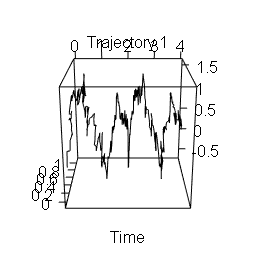
\includegraphics[width=1\linewidth]{../img/3d_1.png}} \\
	\end{minipage}
	\hfill
	\begin{minipage}[h]{0.47\linewidth}
		\center{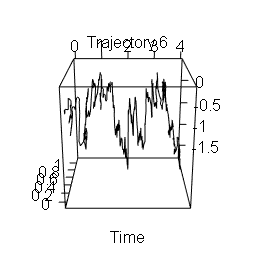
\includegraphics[width=1\linewidth]{../img/3d_6.png}} \\
	\end{minipage}
	\vfill
	\begin{minipage}[h]{0.47\linewidth}
		\center{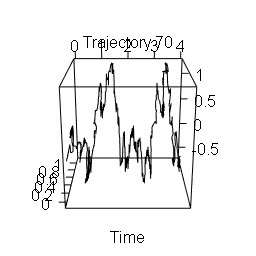
\includegraphics[width=1\linewidth]{../img/3d_70.png}}  \\
	\end{minipage}
	\hfill
	\begin{minipage}[h]{0.47\linewidth}
		\center{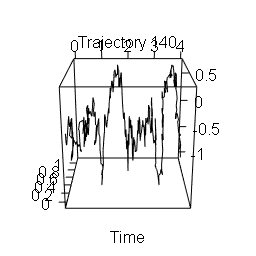
\includegraphics[width=1\linewidth]{../img/3d_140.png}}  \\
	\end{minipage}
\end{figure}


Далее, для этих же траекторий построим классические графики броуновского движения:
\begin{figure}[H]
	\begin{minipage}[h]{.7\linewidth}
		\center{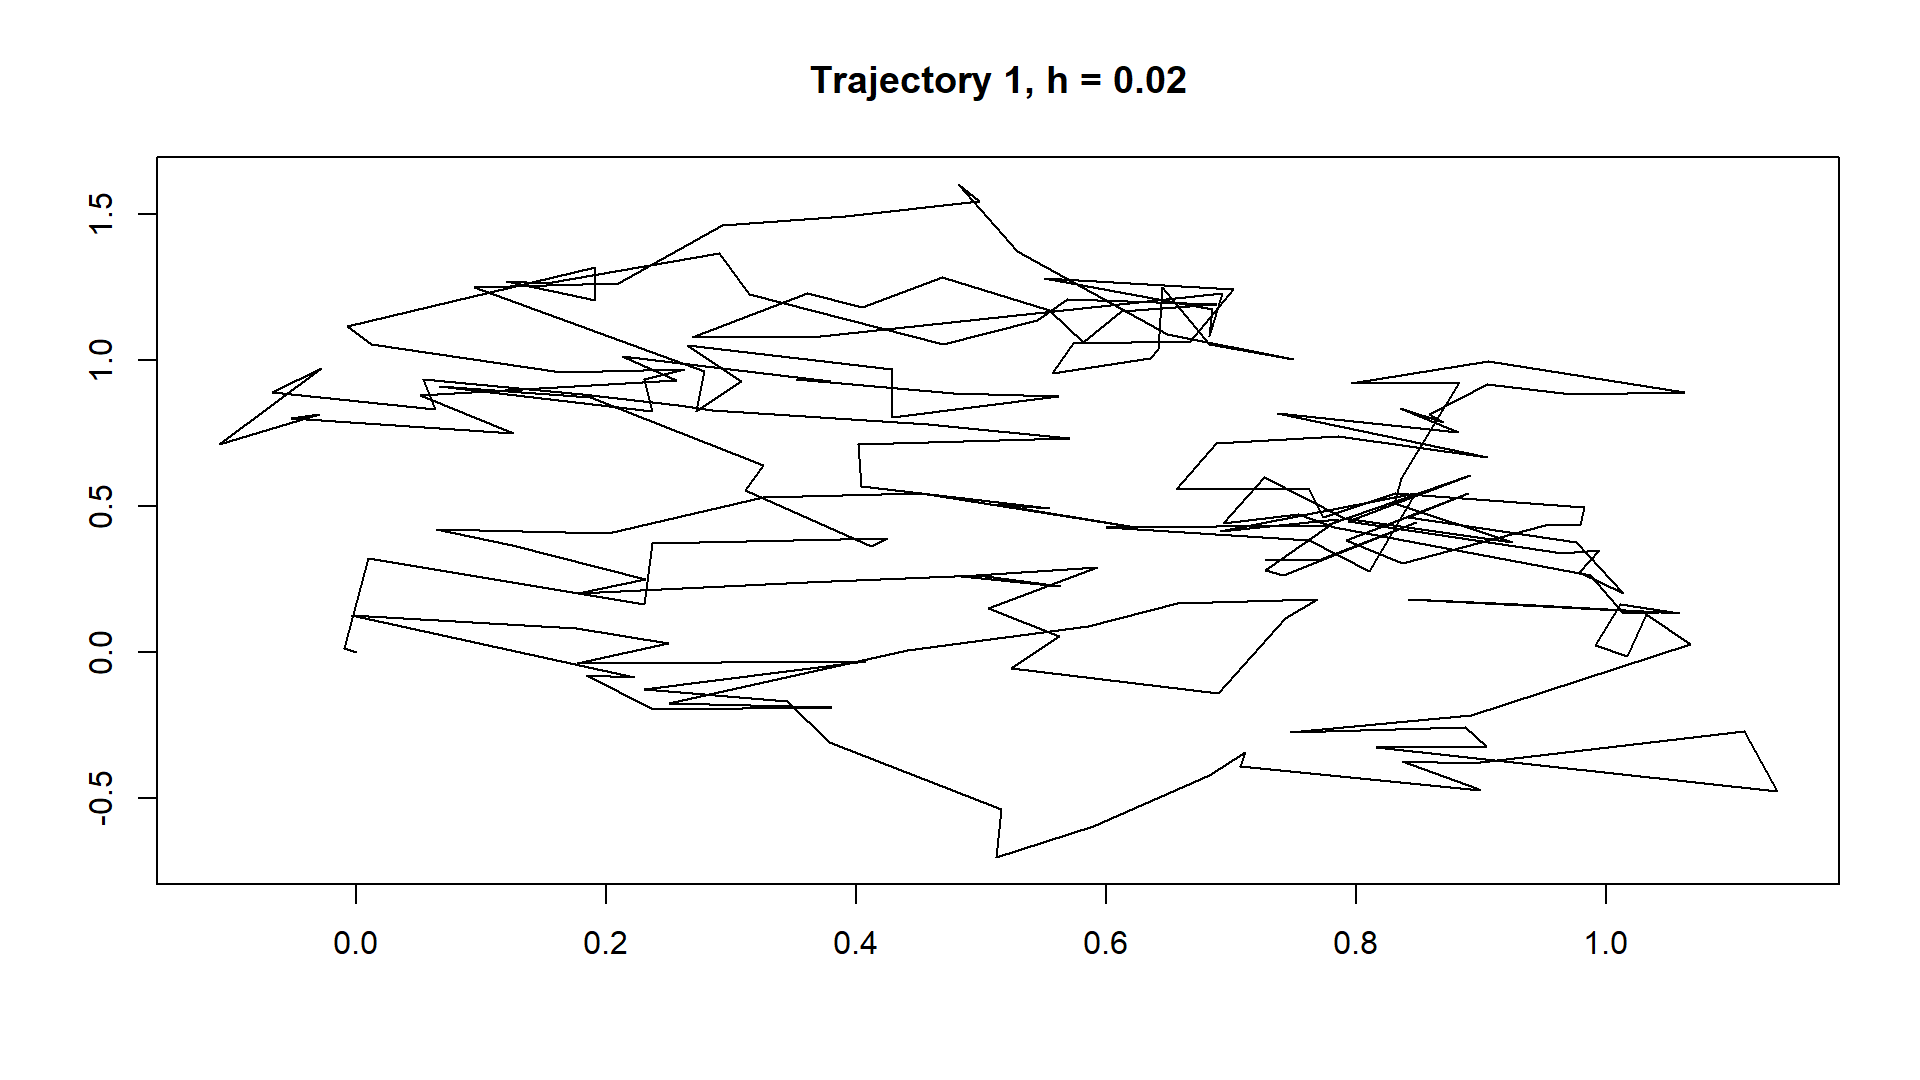
\includegraphics[width=1\linewidth]{../img/2d_1.png}} \\
	\end{minipage}
	\begin{minipage}[h]{.7\linewidth}
		\center{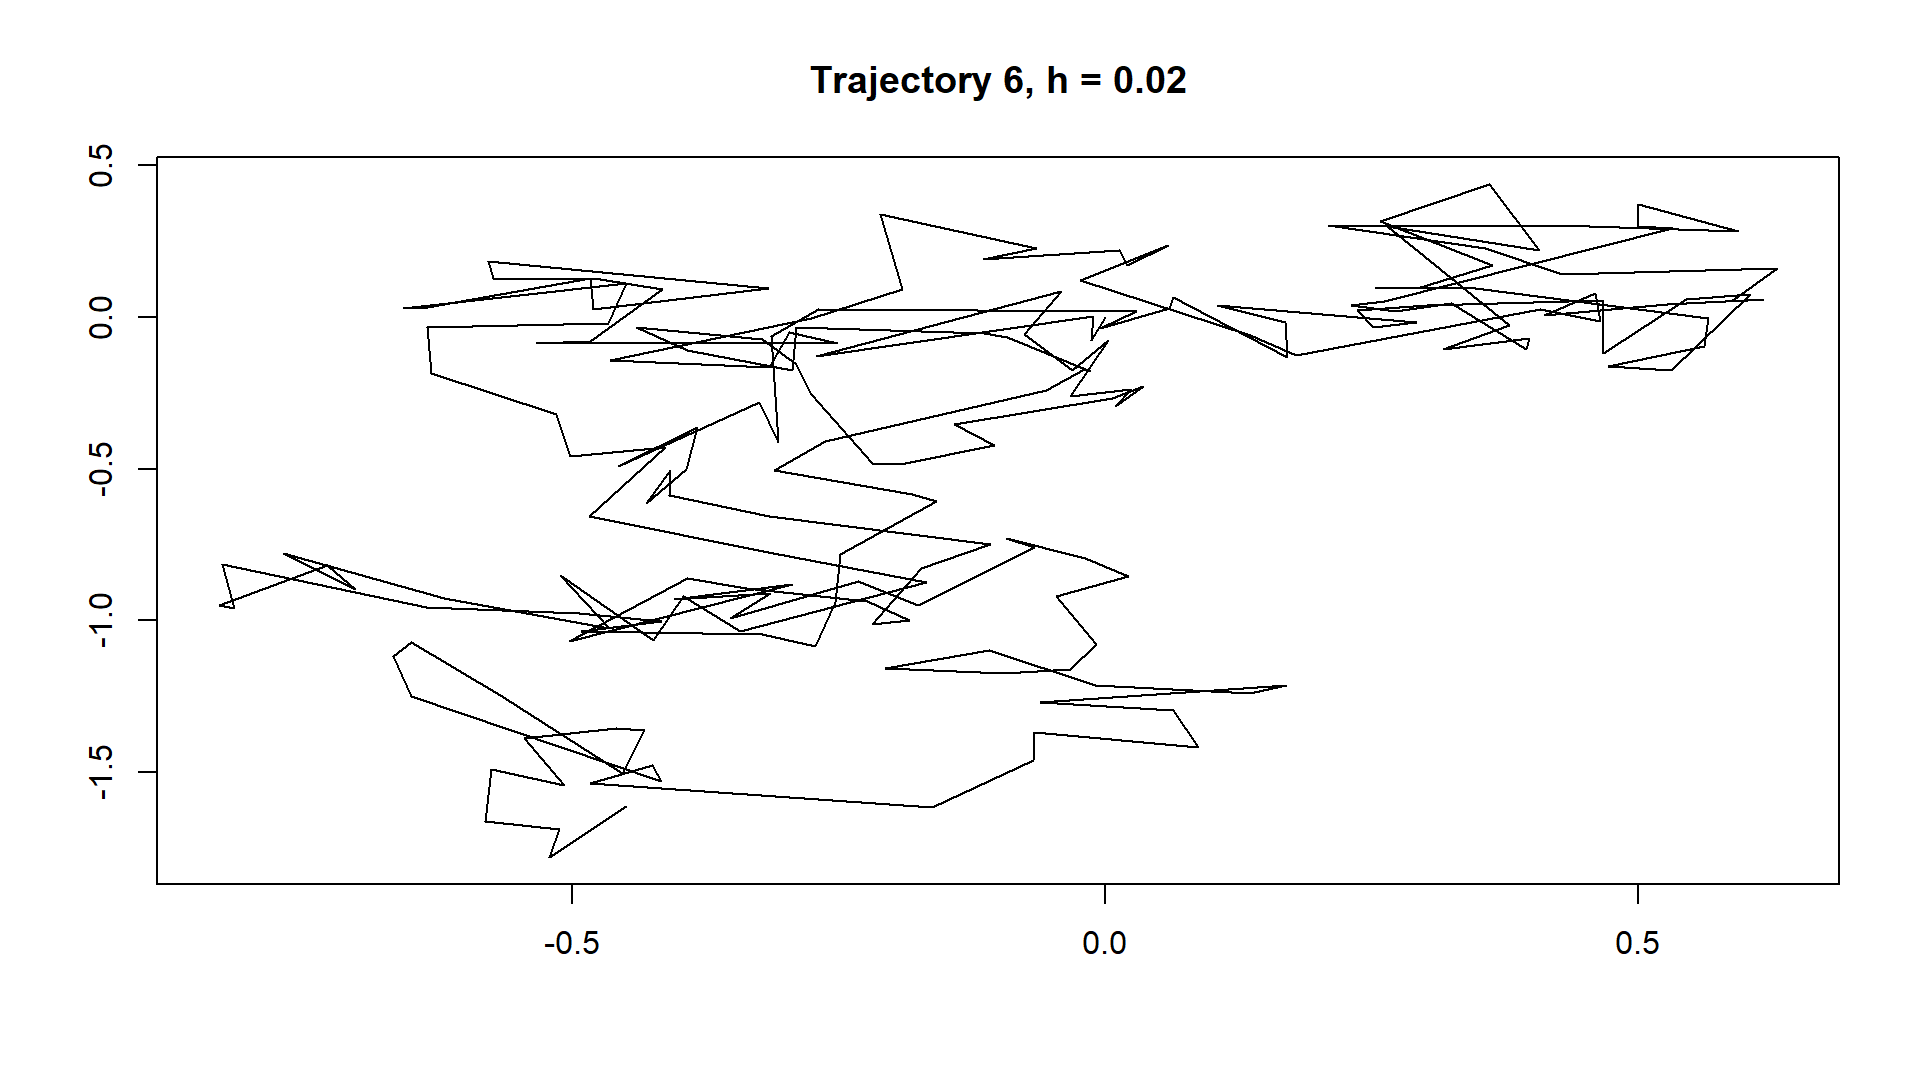
\includegraphics[width=1\linewidth]{../img/2d_6.png}} \\
	\end{minipage}
	\begin{minipage}[h]{.7\linewidth}
		\center{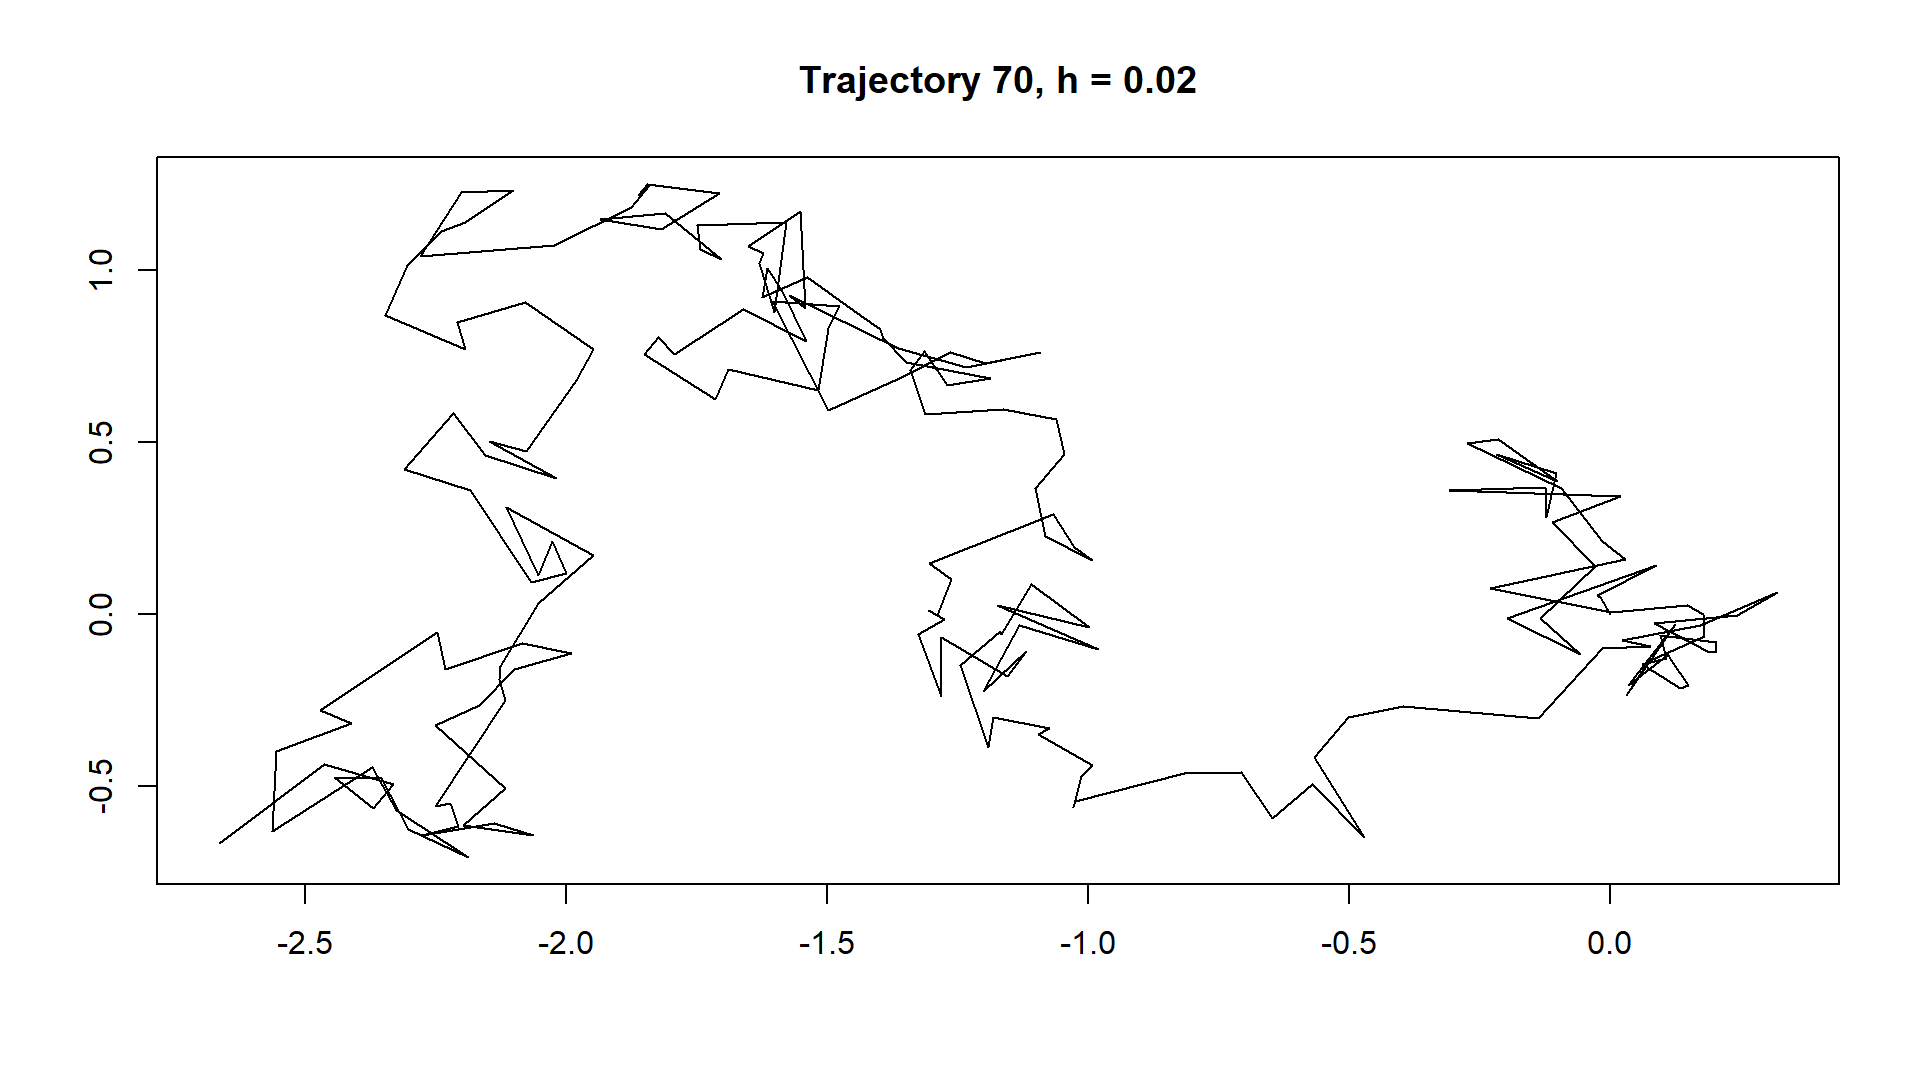
\includegraphics[width=1\linewidth]{../img/2d_70.png}}  \\
	\end{minipage}
	\begin{minipage}[h]{.7\linewidth}
		\center{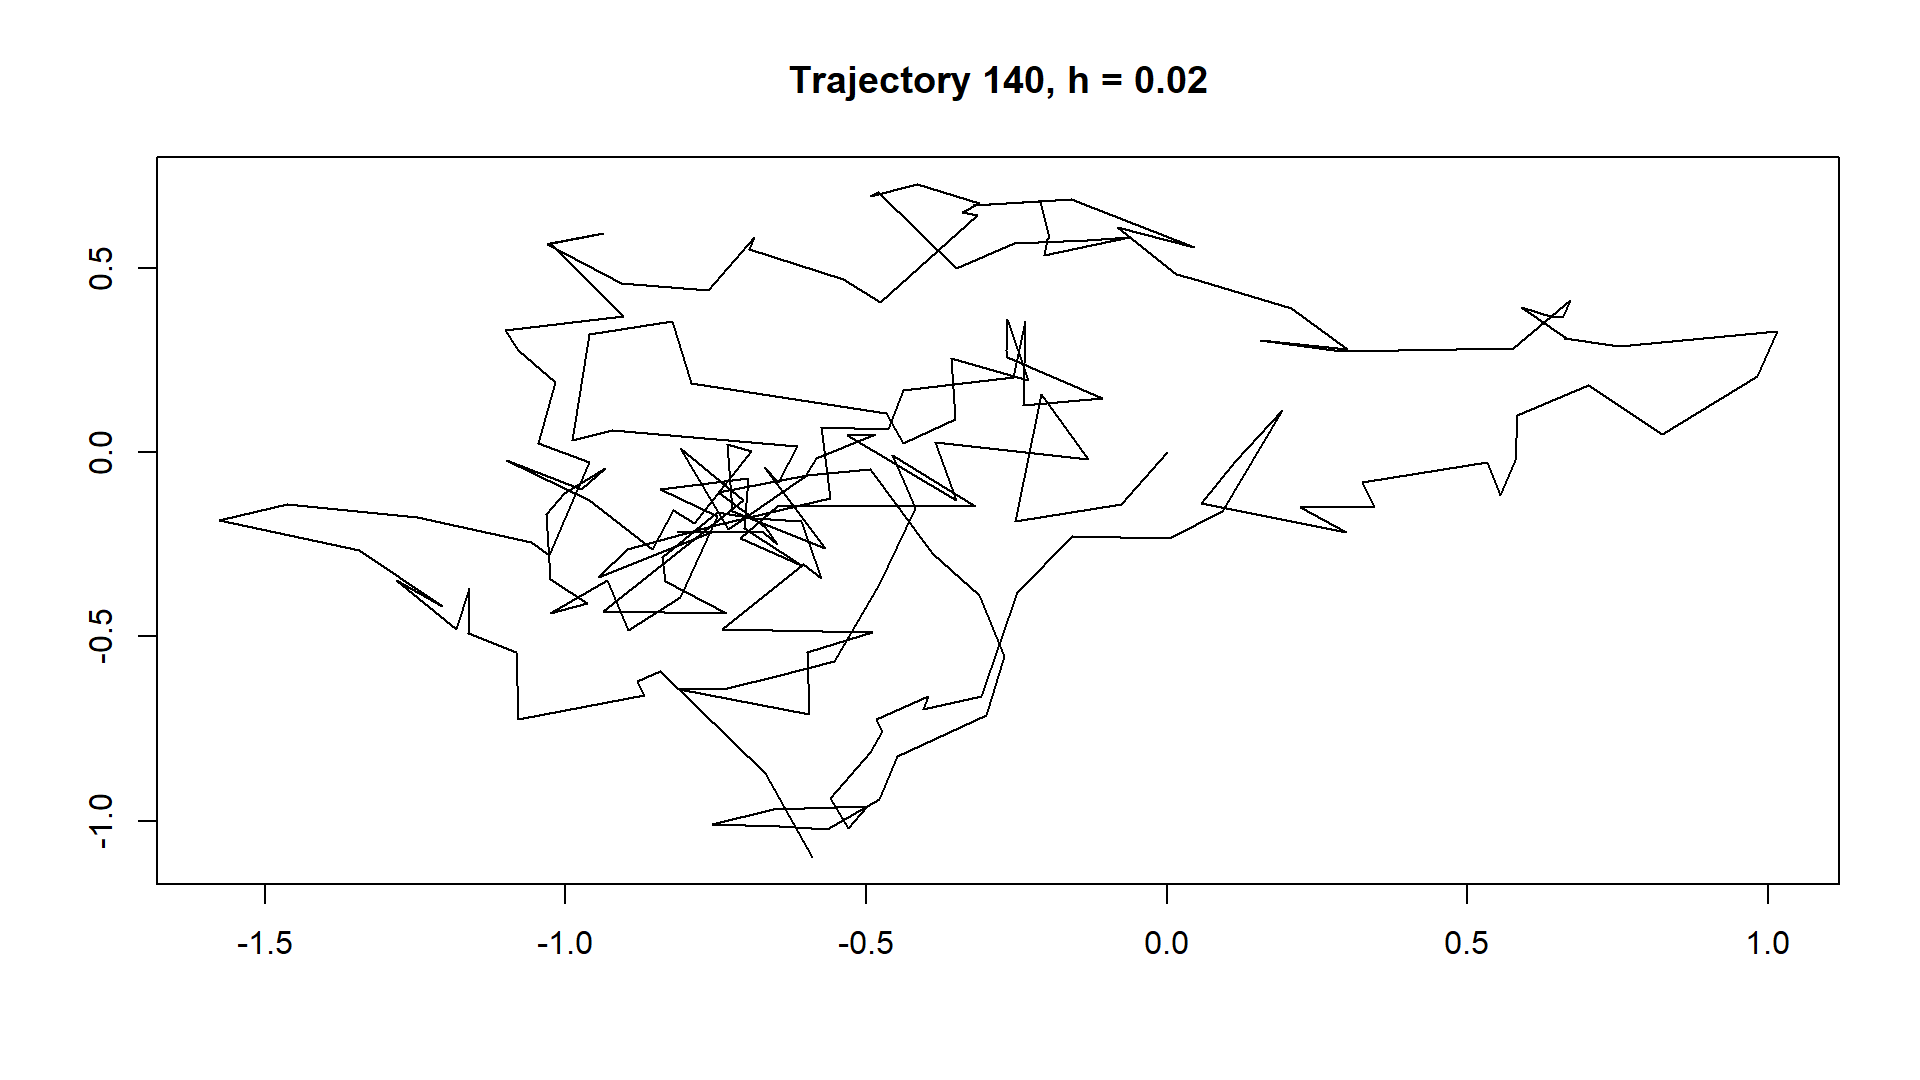
\includegraphics[width=1\linewidth]{../img/2d_140.png}}  \\
	\end{minipage}
\end{figure}



\pagebreak


\subsection{Вычисление характиристик двумерного винеровского процесса}

\subsubsection{Вариации компонент. Среднее значение вариации}

Найдём вариации компонент  $\left(\sum\limits_{k}\left|W_{(k+1) h}^{(1)}-W_{k h}^{(1)}\right|, \sum\limits_{k}\left|W_{(k+1) h}^{(2)}-W_{k h}^{(2)}\right|\right)$:
\begin{minted}{R}
> var_foo <- function(y)
+ {
+   sum(abs(diff(y)))
+ }
> 
> vars <- t(sapply(pairs.list, function(x) apply(x, 2, var_foo)))
\end{minted}


Выведем на печать вариации компонент для первых и последних пяти траекторий:
\begin{minted}{R}
> head(vars,5)
	  [,1]     [,2]
[1,] 17.46365 18.10675
[2,] 16.82400 16.25767
[3,] 17.39559 16.03837
[4,] 17.33865 15.00066
[5,] 16.05115 16.93480
> tail(vars,5)
	  [,1]     [,2]
[156,] 19.99023 17.77190
[157,] 16.35341 16.54479
[158,] 16.62718 17.14943
[159,] 17.45334 18.07495
[160,] 16.78373 17.36628
\end{minted}


Тогда среднее значение вариации $\left(\operatorname{Var}^{(1)}(h), \operatorname{Var}^{(2)}(h)\right)$ по всем траекториям:

\begin{minted}{R}
> mean_vars <- colMeans(vars)
> mean_vars
[1] 17.01906 16.91866
\end{minted}

\pagebreak

\subsubsection{Суммы квадратов приращений. Среднее значение суммы квадратов приращений}

Найдём суммы квадратов приращений компонент \\${\left(\sum\limits_{k}\left|W_{(k+1) h}^{(1)}-W_{k h}^{(1)}\right|^2, \sum\limits_{k}\left|W_{(k+1) h}^{(2)}-W_{k h}^{(2)}\right|^2\right)}$:

\begin{minted}{R}
> sq.var_foo <- function(y)
+ {
+   sum(abs(diff(y))^2)
+ }
> 
> sq.vars <- t(sapply(pairs.list, function(x) apply(x, 2, sq.var_foo)))
\end{minted}


Выведем на печать вариации компонент для первых и последних пяти траекторий:
\begin{minted}{R}
> head(sq.vars,5)
	  [,1]     [,2]
[1,] 2.333261 2.598706
[2,] 2.208715 2.124458
[3,] 2.313816 2.017766
[4,] 2.368920 1.849391
[5,] 1.961947 2.345290
> tail(sq.vars,5)
	  [,1]     [,2]
[156,] 3.147324 2.232487
[157,] 2.128623 2.094030
[158,] 2.105166 2.304816
[159,] 2.478495 2.442681
[160,] 2.163211 2.254925
\end{minted}

Найдём среднее значение этих сумм $(\operatorname{SqVar}^{(1)}(h), \operatorname{SqVar}^{(2)}(h))$:

\begin{minted}{R}
> mean_sq.vars <- colMeans(vars)
> mean_sq.vars
[1] 2.285641 2.243726
\end{minted}


\pagebreak

\subsection{Рассмотрение уменьшенного вдвое шага $h$}\label{4}
Для более детального изучения картины поведения броуновского движения уменьшим шаг $h$ вдвое до $\tilde{h} = \frac{h}{2} = 0.01$. Проделаем описанные выше действия для получившегося двумерного винеровского процесса.

Найдём вариации компонент $\left(\sum\limits_{k}\left|W_{(k+1) \tilde{h}}^{(1)}-W_{k \tilde{h}}^{(1)}\right|, \sum\limits_{k}\left|W_{(k+1) \tilde{h}}^{(2)}-W_{k \tilde{h}}^{(2)}\right|\right)$:

\begin{minted}{R}
> vars.extnd <- t(sapply(pairs.extnd.list, 
+	function(x) apply(x, 2, var_foo)))
> head(vars.extnd,5)
	  [,1]     [,2]
[1,] 24.26126 25.06274
[2,] 25.18078 23.63542
[3,] 23.54455 24.56995
[4,] 23.46042 23.20730
[5,] 22.35894 22.91436
> tail(vars.extnd,5)
	  [,1]     [,2]
[156,] 26.86954 23.84102
[157,] 23.28283 22.33214
[158,] 25.28249 24.57040
[159,] 23.64685 25.76409
[160,] 24.12964 23.42405
\end{minted}

А так же среднее значение вариации $\left(\operatorname{Var}^{(1)}(\tilde{h}), \operatorname{Var}^{(2)}(\tilde{h})\right)$:

\begin{minted}{R}
> mean_vars.extnd <- colMeans(vars.extnd)
> mean_vars.extnd
[1] 24.02536 23.96380
\end{minted}

Далее ищем суммы квадратов приращений компонент \\ $\left(\sum\limits_{k}\left|W_{(k+1) \tilde{h}}^{(1)}-W_{k \tilde{h}}^{(1)}\right|^2, \sum\limits_{k}\left|W_{(k+1) \tilde{h}}^{(2)}-W_{k \tilde{h}}^{(2)}\right|^2\right)$:

\begin{minted}{R}
> sq.vars.extnd  <- t(sapply(pairs.extnd.list, 
+	function(x) apply(x, 2, sq.var_foo)))
> head(sq.vars.extnd ,5)
[,1]     [,2]
[1,] 2.326814 2.470255
[2,] 2.413601 2.326623
[3,] 2.106365 2.234015
[4,] 2.244770 2.045897
[5,] 1.967547 2.112295
> tail(sq.vars.extnd ,5)
[,1]     [,2]
[156,] 2.782908 2.147537
[157,] 2.137992 1.946296
[158,] 2.447775 2.410783
[159,] 2.224500 2.576072
[160,] 2.201613 2.195686
\end{minted}

А так же среднее значение этих сумм $(\operatorname{SqVar}^{(1)}(\tilde{h}), \operatorname{SqVar}^{(2)}(\tilde{h}))$

\begin{minted}{R}
> mean_sq.vars.extnd  <- colMeans(vars.extnd )
> mean_sq.vars.extnd 
[1] 2.266860 2.257994
\end{minted}

Можем сравнить полученные средние для двух значений $h$. Первый и третий столбец соответствуют $h = 0.02$, а второй и четвёртый -- $\tilde{h} = 0.01$:

\begin{minted}{R}
> compare_table <- data.table(mean_vars = mean_vars,
+                             mean_vars.extnd = mean_vars.extnd,
+                             mean_sq.vars = mean_sq.vars,
+                             mean_sq.vars.extnd = mean_sq.vars.extnd)
> compare_table
mean_vars mean_vars.extnd mean_sq.vars mean_sq.vars.extnd
1:  17.01906        24.02536     2.285641           2.266860
2:  16.91866        23.96380     2.243726           2.257994
\end{minted}

Или в относительных величинах:

\begin{minted}{R}
> compare_table.rel <- data.table(compare_table[,1] / compare_table[,2],
+                                 compare_table[,3] / compare_table[,4])
> compare_table.rel
mean_vars mean_sq.vars
1: 0.7083788    1.0082851
2: 0.7060092    0.9936808
\end{minted}

Видим, что отличия в средних значениях суммы квадратов приращений компонент существенно меньше, чем отличия у средних значений вариаций компонент.


Наконец построим графики:
\begin{figure}[H]
	\begin{minipage}[h]{.7\linewidth}
		\center{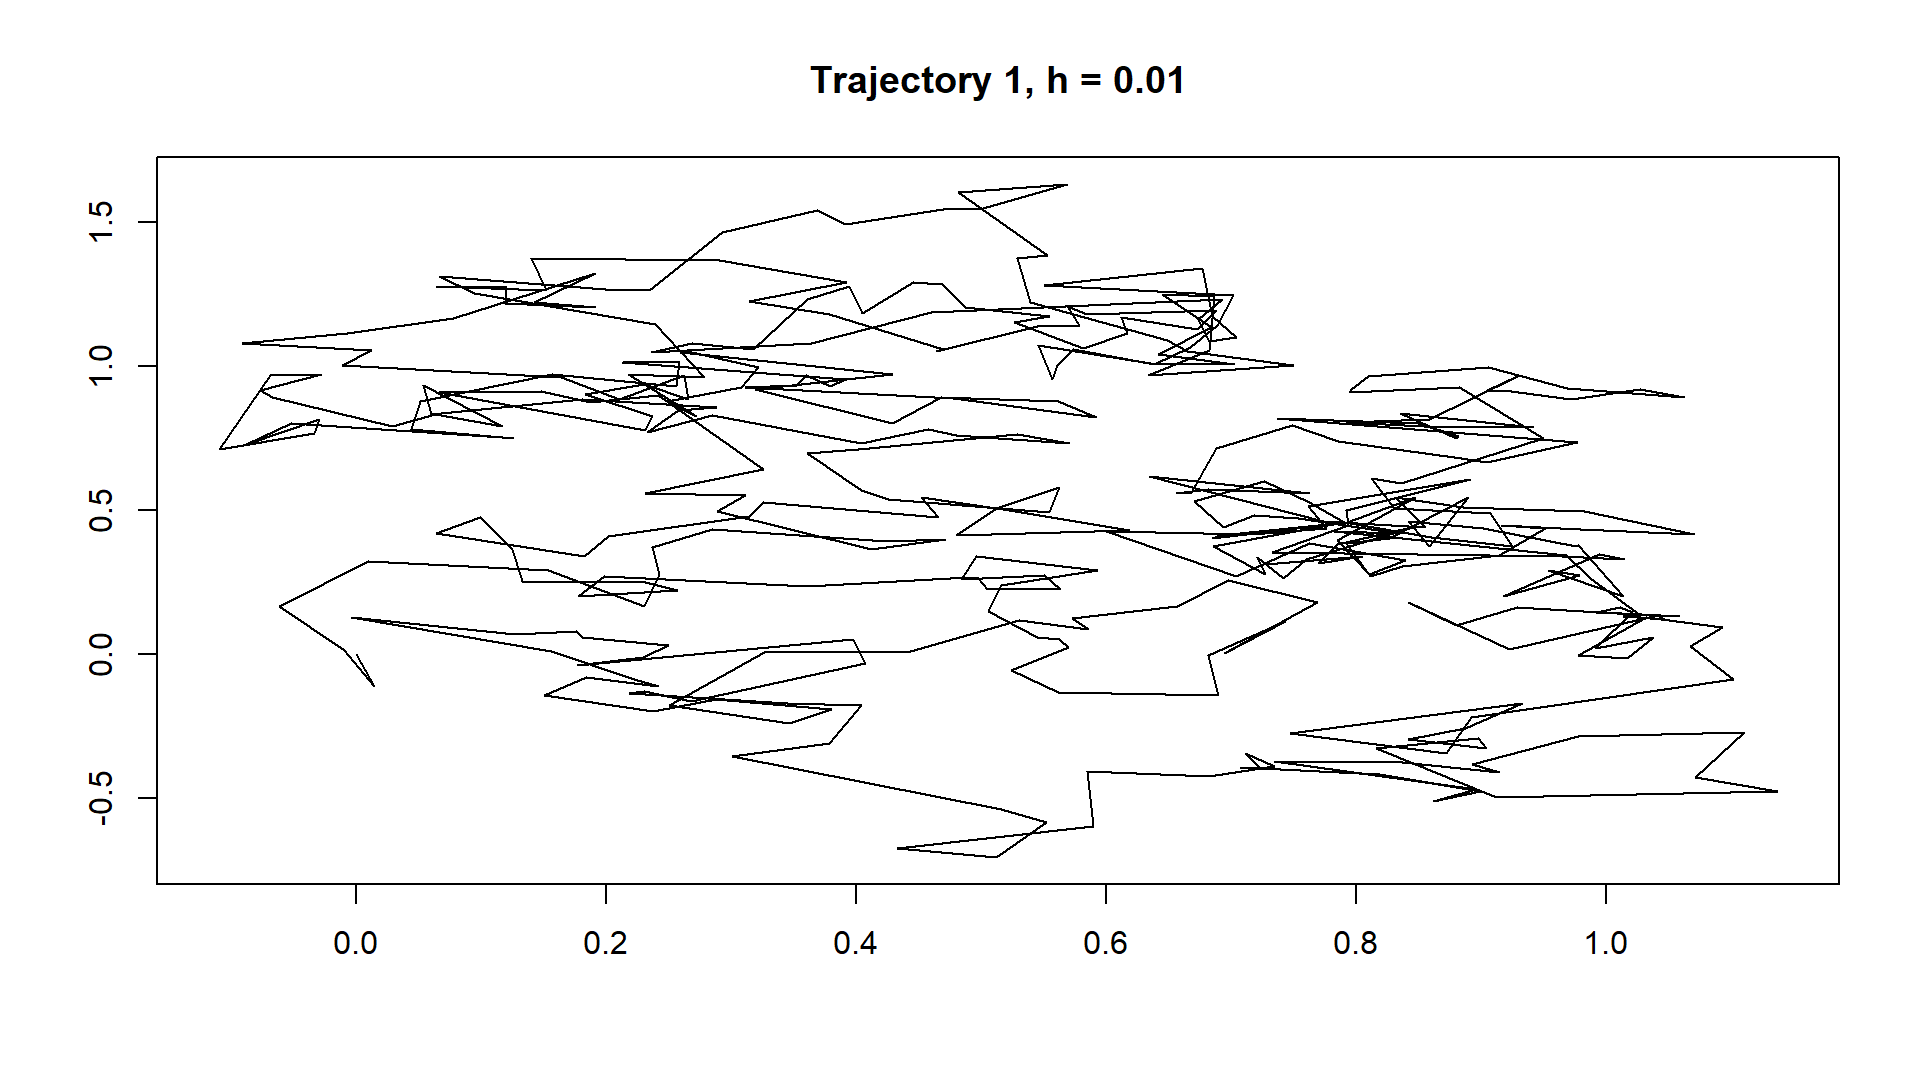
\includegraphics[width=1\linewidth]{../img/2d_1_ext.png}} \\
	\end{minipage}
	\begin{minipage}[h]{.7\linewidth}
		\center{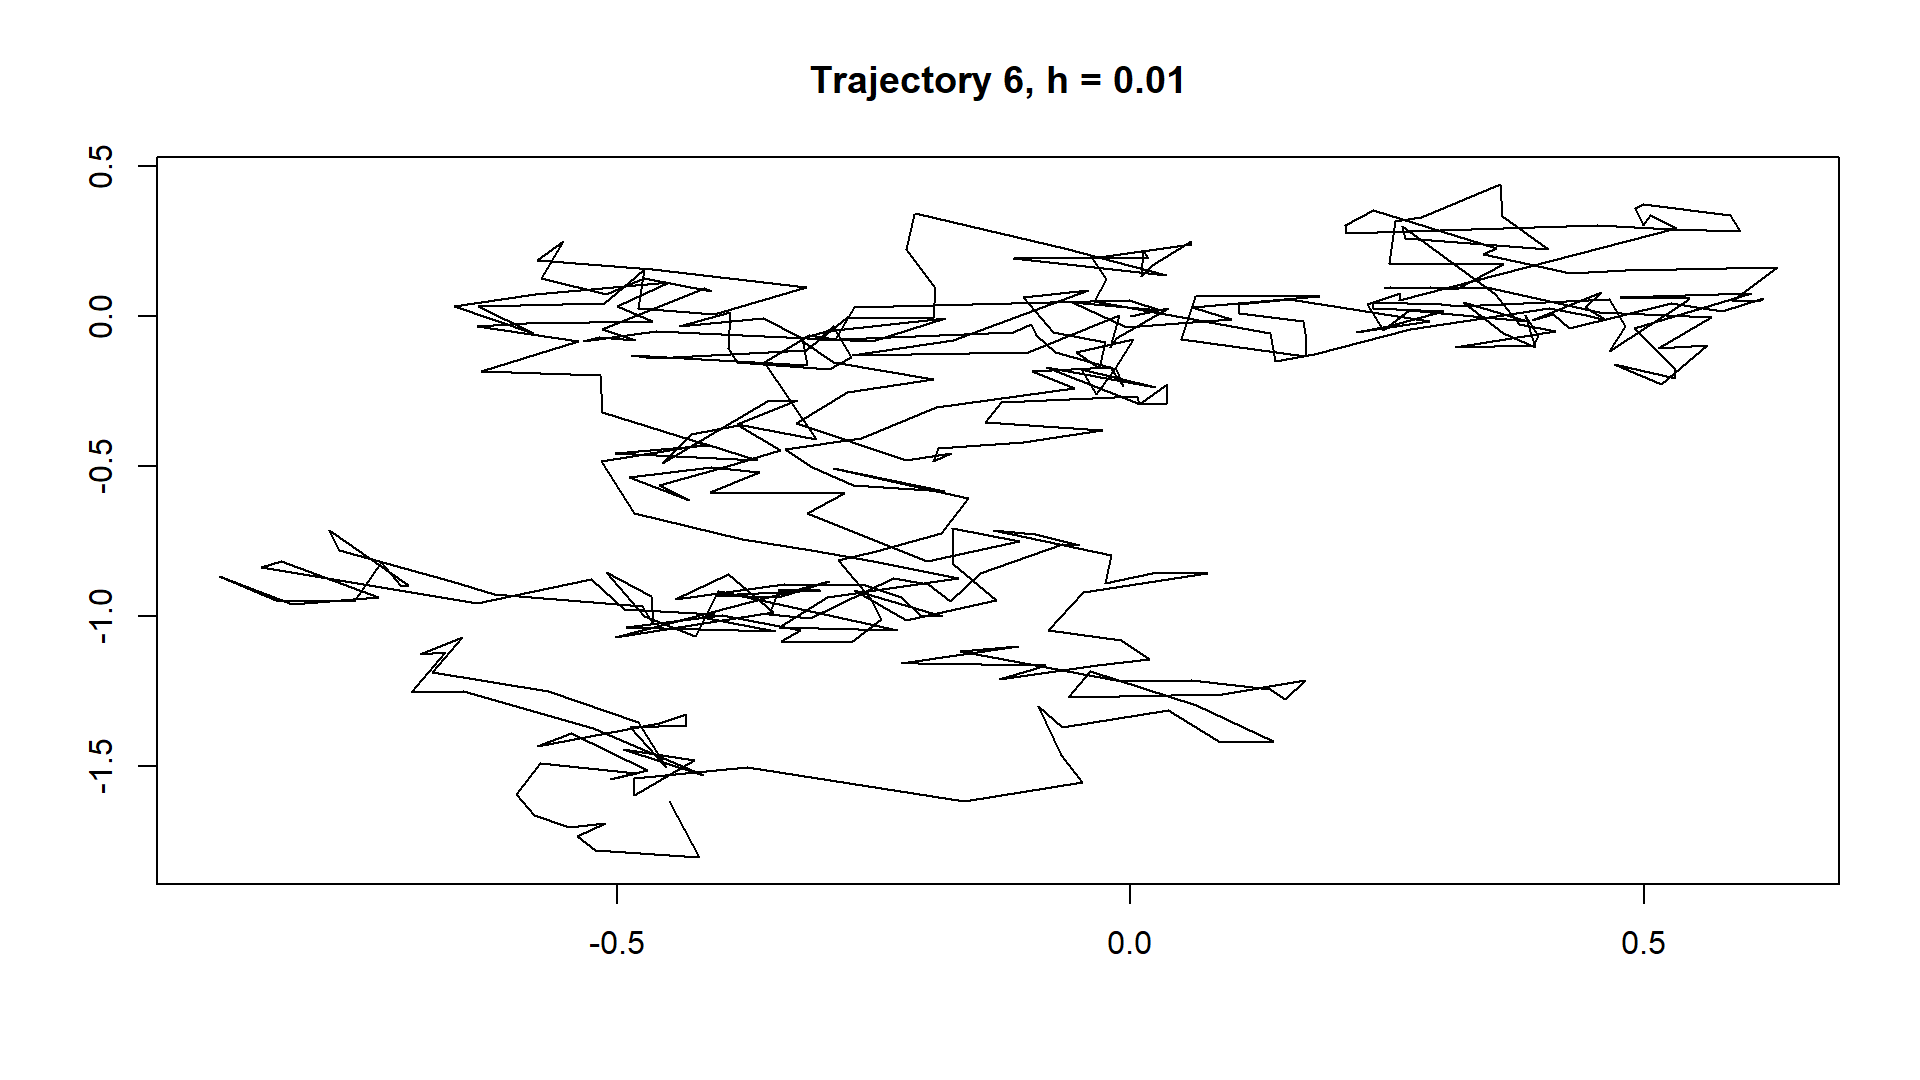
\includegraphics[width=1\linewidth]{../img/2d_6_ext.png}} \\
	\end{minipage}
	\begin{minipage}[h]{.7\linewidth}
		\center{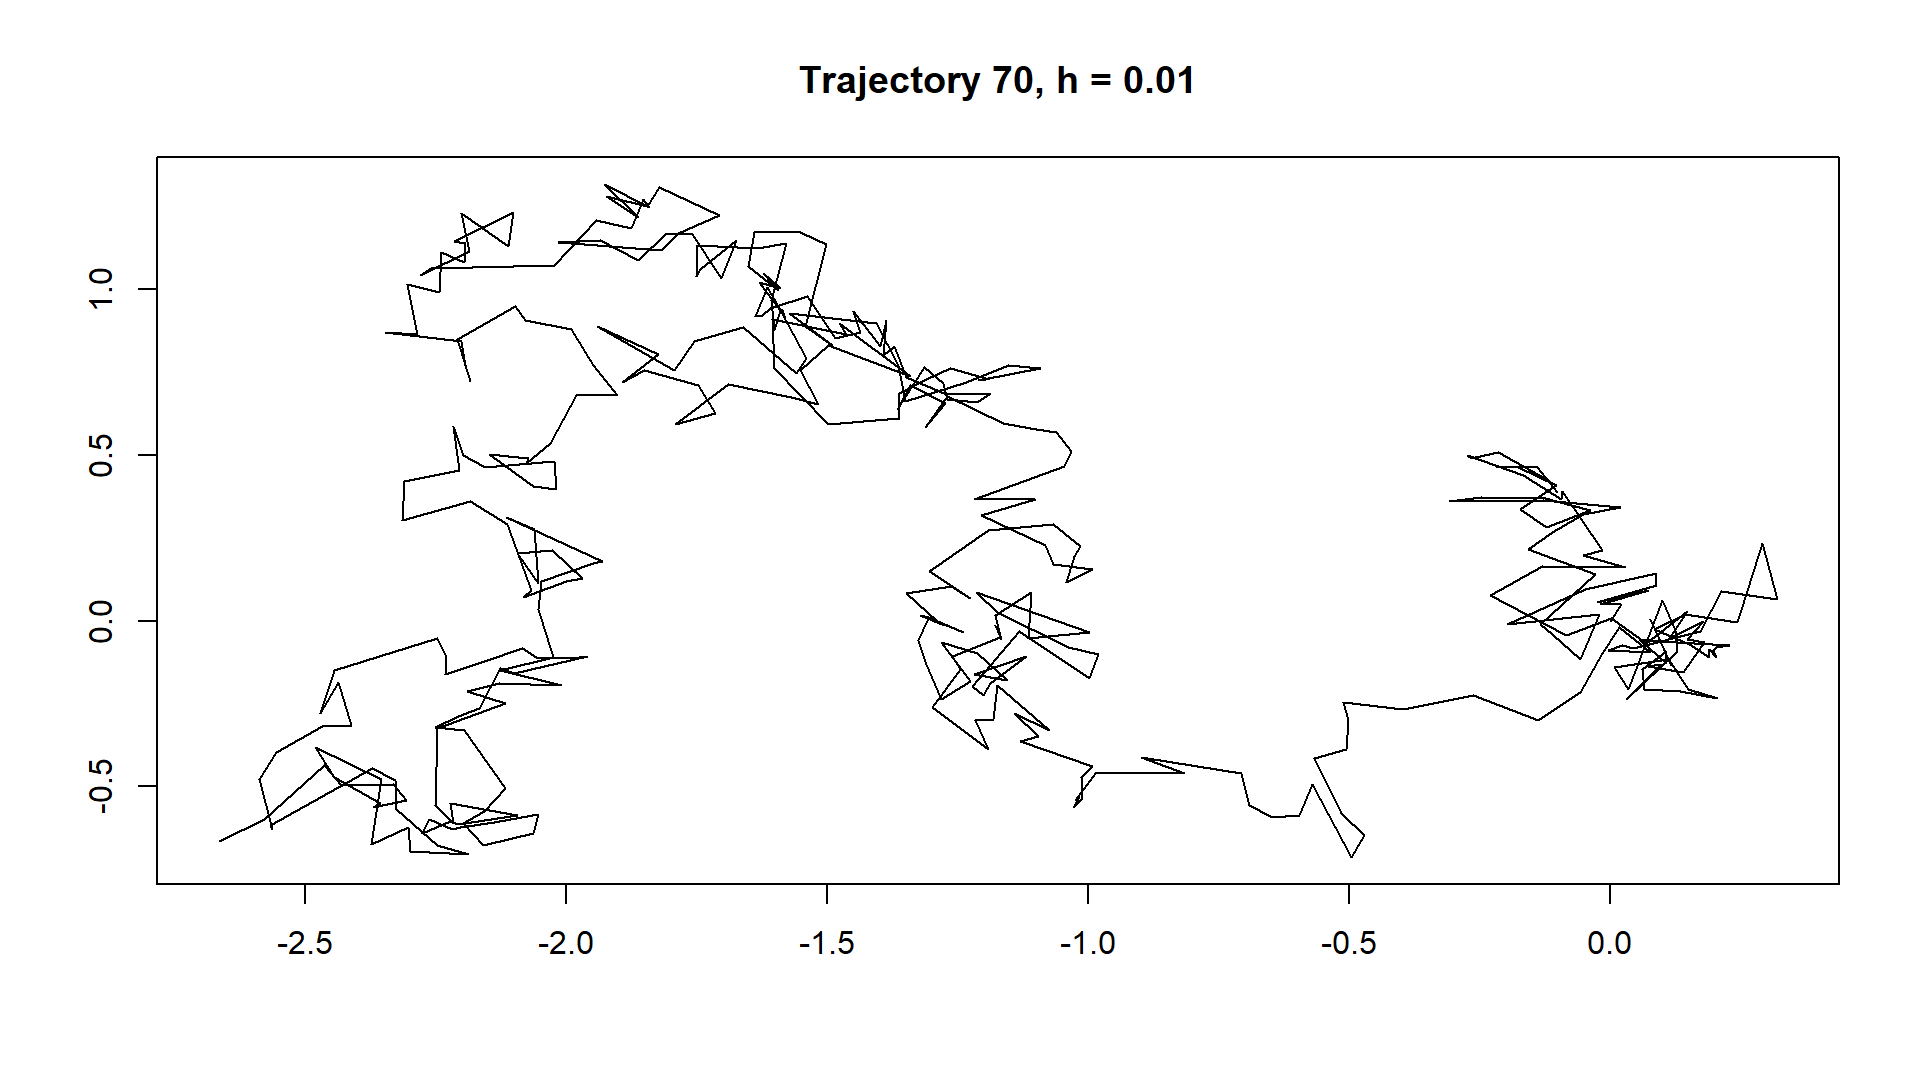
\includegraphics[width=1\linewidth]{../img/2d_70_ext.png}}  \\
	\end{minipage}
	\begin{minipage}[h]{.7\linewidth}
		\center{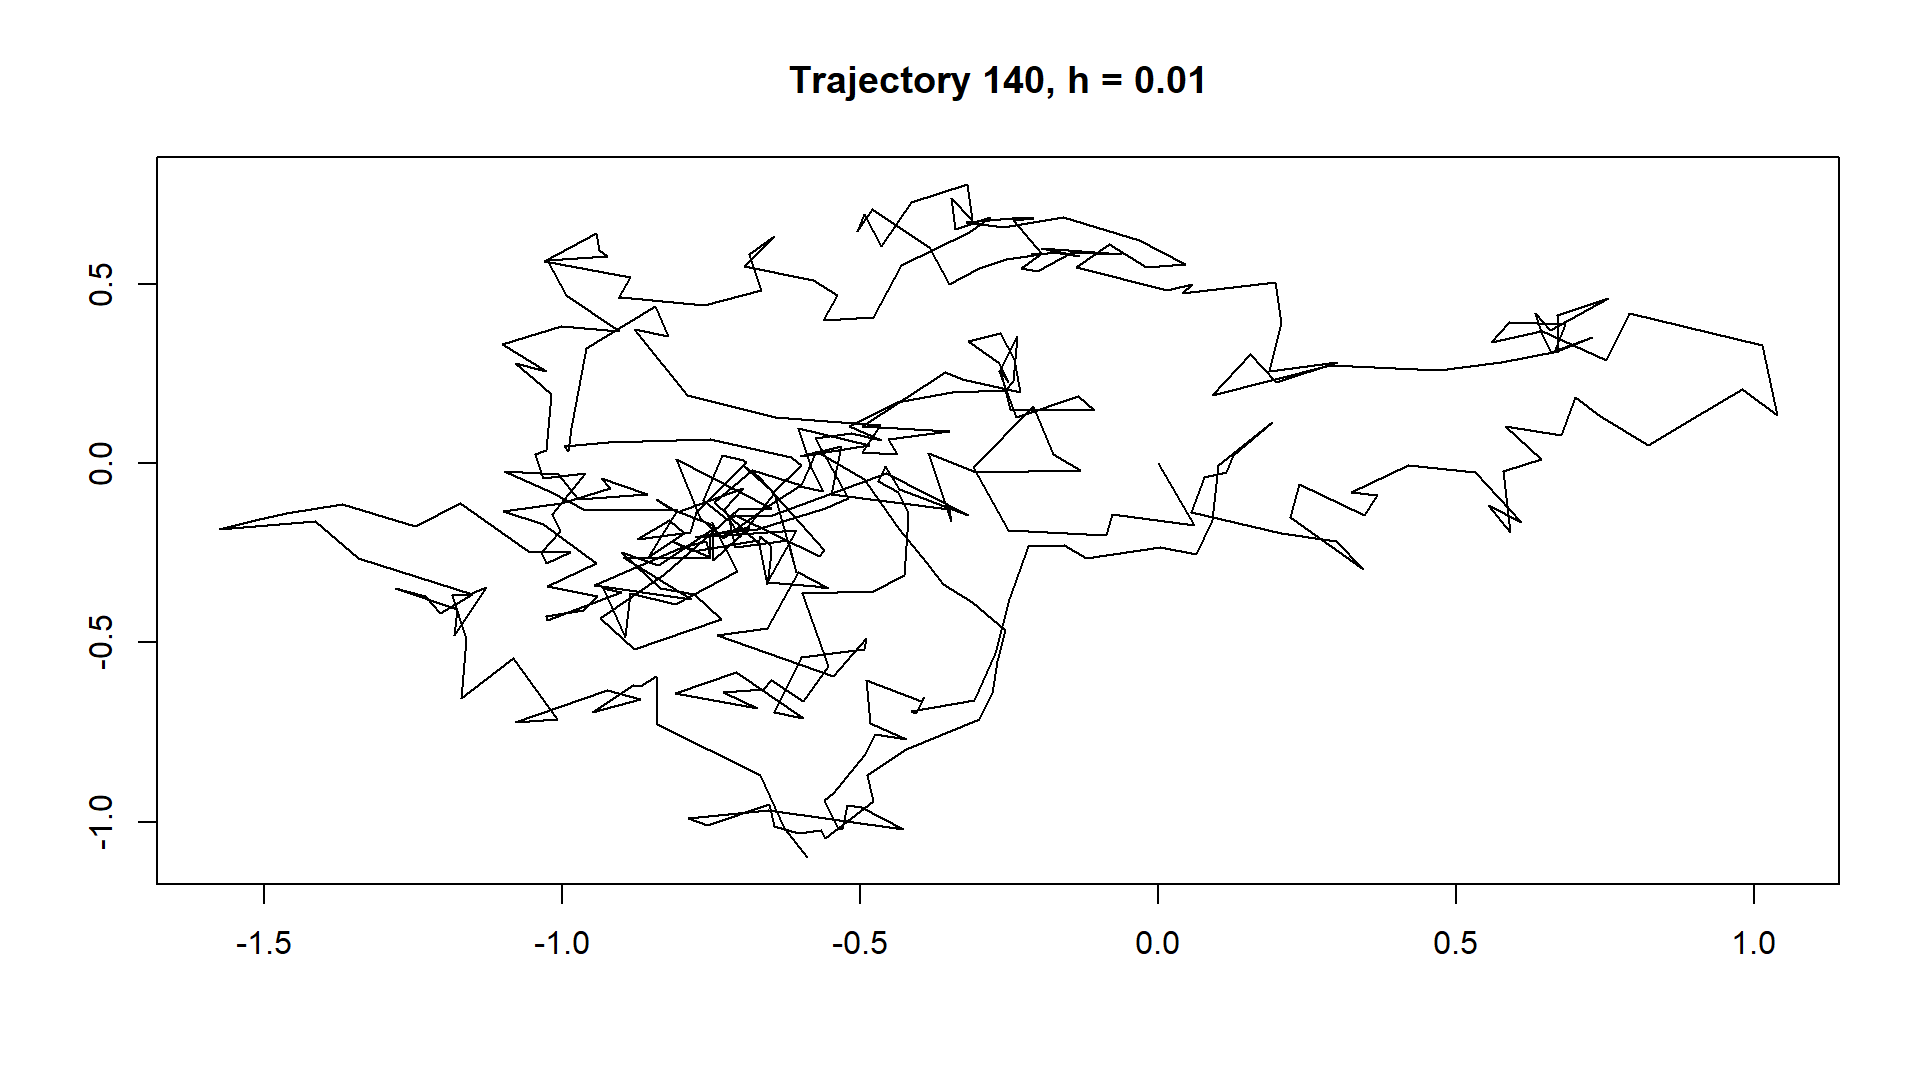
\includegraphics[width=1\linewidth]{../img/2d_140_ext.png}}  \\
	\end{minipage}
\end{figure}


\pagebreak

Кроме того, можем построить совмещённые графики для соответствующих траекторий при $h = 0.02$ и $\tilde{h} = 0.01$.

\begin{figure}[H]
	\begin{minipage}[h]{1\linewidth}
		\center{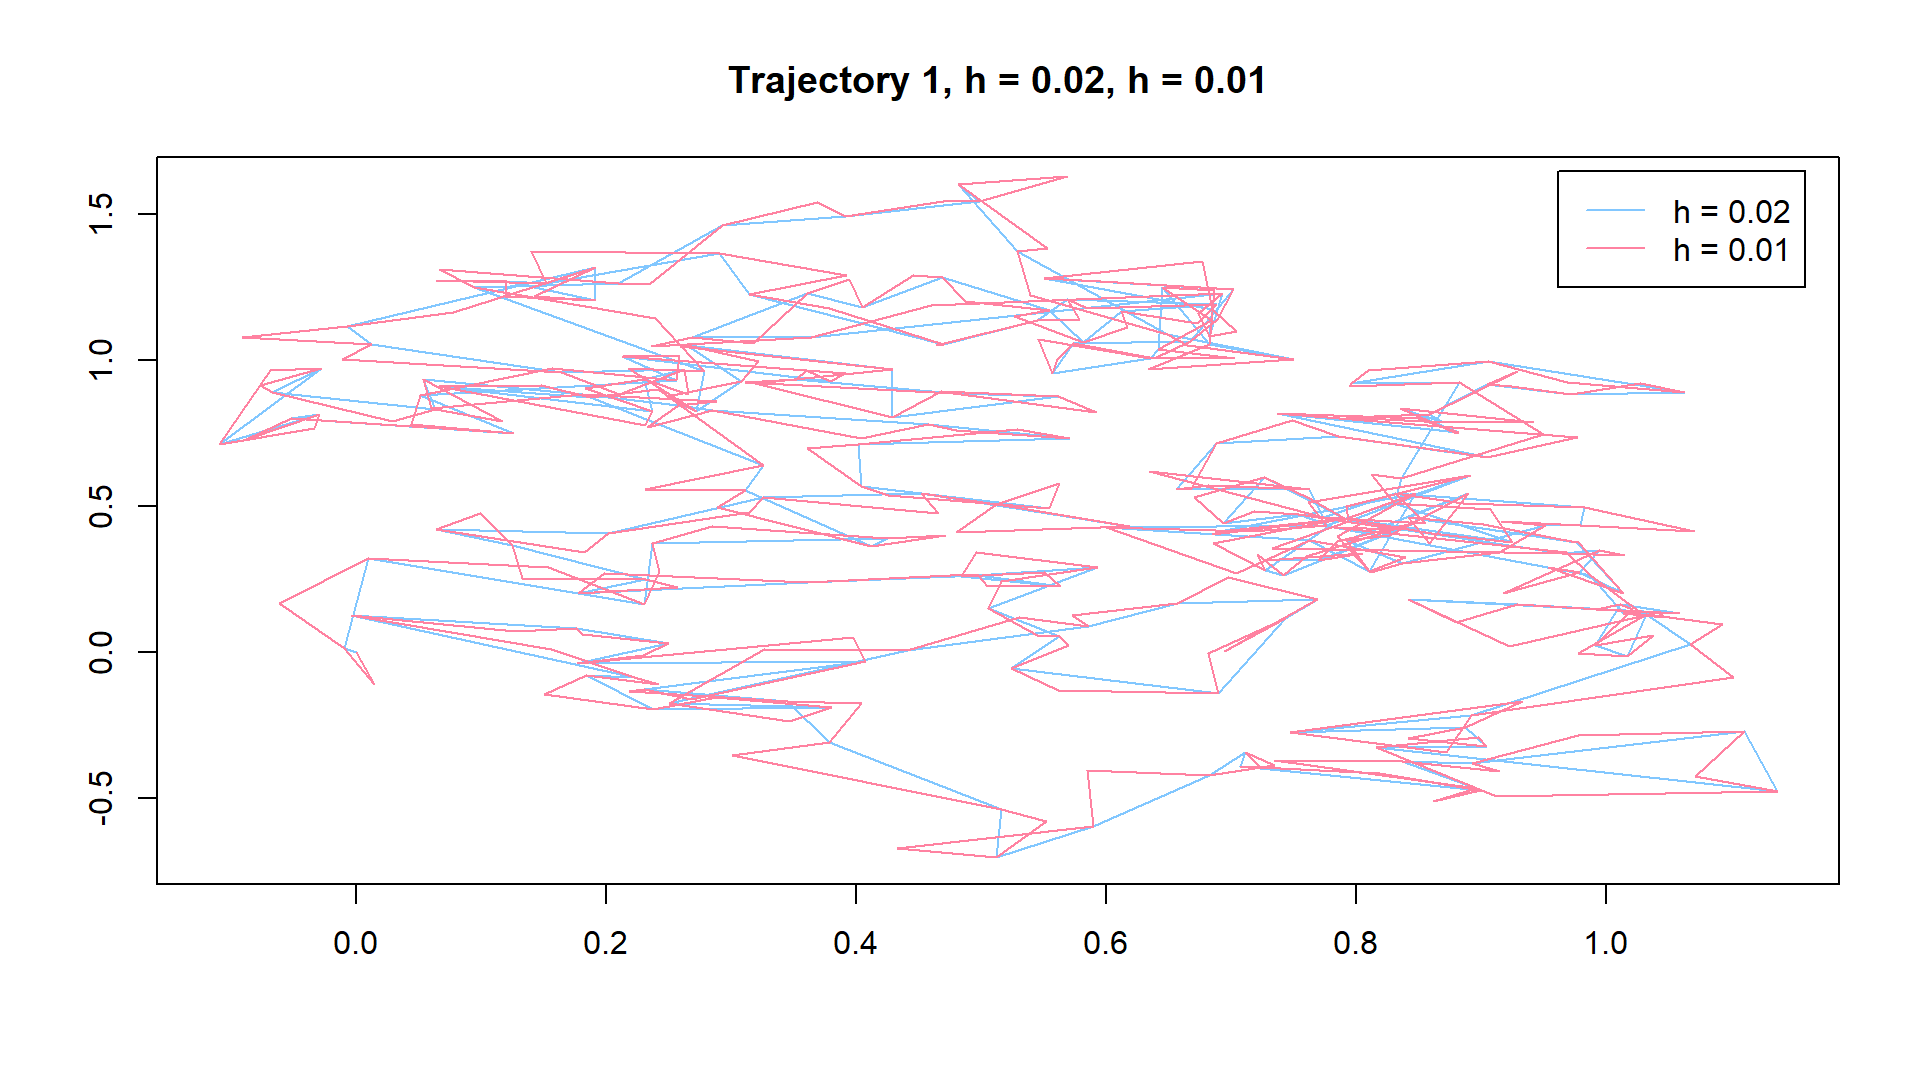
\includegraphics[width=.95\linewidth]{../img/2d_1_1.png}}  \\
	\end{minipage}
\end{figure}



В связи с большим количеством точек график выглядит не очень информативным. Рассмотрим в приближении несколько точек детальнее:

\begin{figure}[H]
	\begin{minipage}[h]{1\linewidth}
		\center{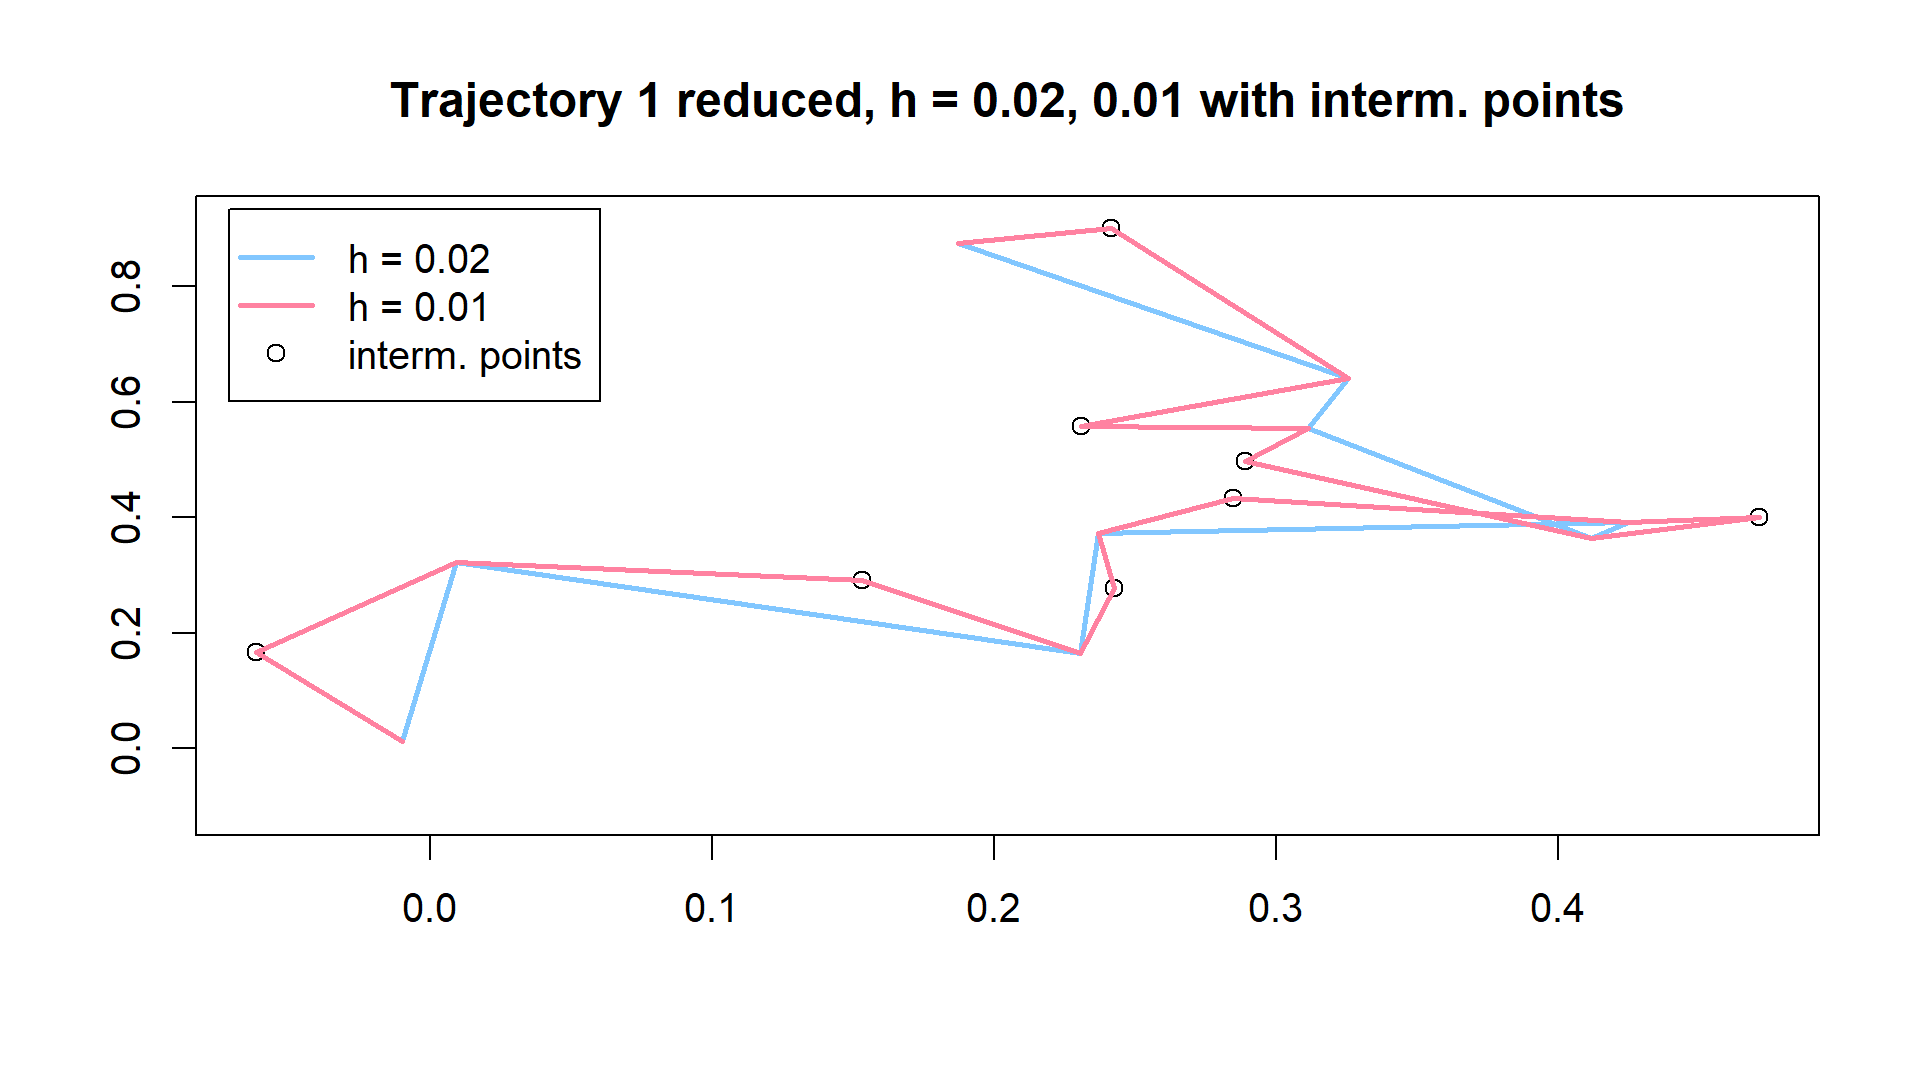
\includegraphics[width=.95\linewidth]{../img/2d_1_1_reduced.png}}  \\
	\end{minipage}
\end{figure}


Теперь можем видеть разницу между траекториями с $h = 0.02$ и ${\tilde{h} = \frac{h}{2} = 0.01}$. Уменьшение в два раза шага позволяет получить <<промежуточные>> точки при рассмотрении броуновского движения частицы.


\subsection{Вероятность достижения уровня $z$ в момент $T$}

Рассчитаем эмпирическую вероятность достижения уровня $z$ в момент $T$. Будем интерпретировать это как количество траекторий, которые в момент времени $T = 4$ находятся за пределами окружности радиуса $z = 2.5$. Это соответствует значению евклидовной метрики на последней точке для каждой траектории. То есть:

\begin{minted}{R}
> euc_metric <- function(y)
+ {
+   sqrt(sum(y[dim(y)[1],]^2))
+ }
> 
> z.sc <- as.numeric(Map(euc_metric, pairs.list))
\end{minted}

Выведем на печать первые и последние 5 элементов полученных значений:
\begin{minted}{R}
> head(z.sc,5)
[1] 0.7919054 0.7308046 1.7206144 1.1162275 1.2255906
> tail(z.sc,5)
[1] 2.0275873 1.5579907 0.7739086 1.5382913 2.5450301
\end{minted}

Теперь можем рассчитать долю траекторий, последняя точка которых находится вне окружности радиуса $z = 2.5$:
\begin{minted}{R}
> pos.sc <- length(z_sc[z_sc > z])
> pos.sc
[1] 42
> z.prob <- pos.sc/((N/2)+1)
> z.prob
[1] 0.2089552
\end{minted}

Значение \mintinline{R}{(N/2)+1} обусловлено особенностями реализации, которые были описаны выше. Длина каждой траектории, как и требуется по условию равняется $\frac{T}{h} + 1 = 200 + 1 = 201$, где дополнительная единица соответствует точке $(0;0)$. Значение \mintinline{R}{N} же равняется $400$, так как оно используется в формировании траекторий \mintinline{R}{pairs.extnd.list} при $\tilde{h} = \frac{h}{2} = 0.01$ для выполнения пункта \ref{4}.


Кроме того, можем изобразить несколько графиков, отражающих взаимное расположение траектории, окружности радиуса $z = 2.5$ и точки, соответствующей последнему положению частицы:



\begin{figure}[H]
	\begin{minipage}[h]{1\linewidth}
		\center{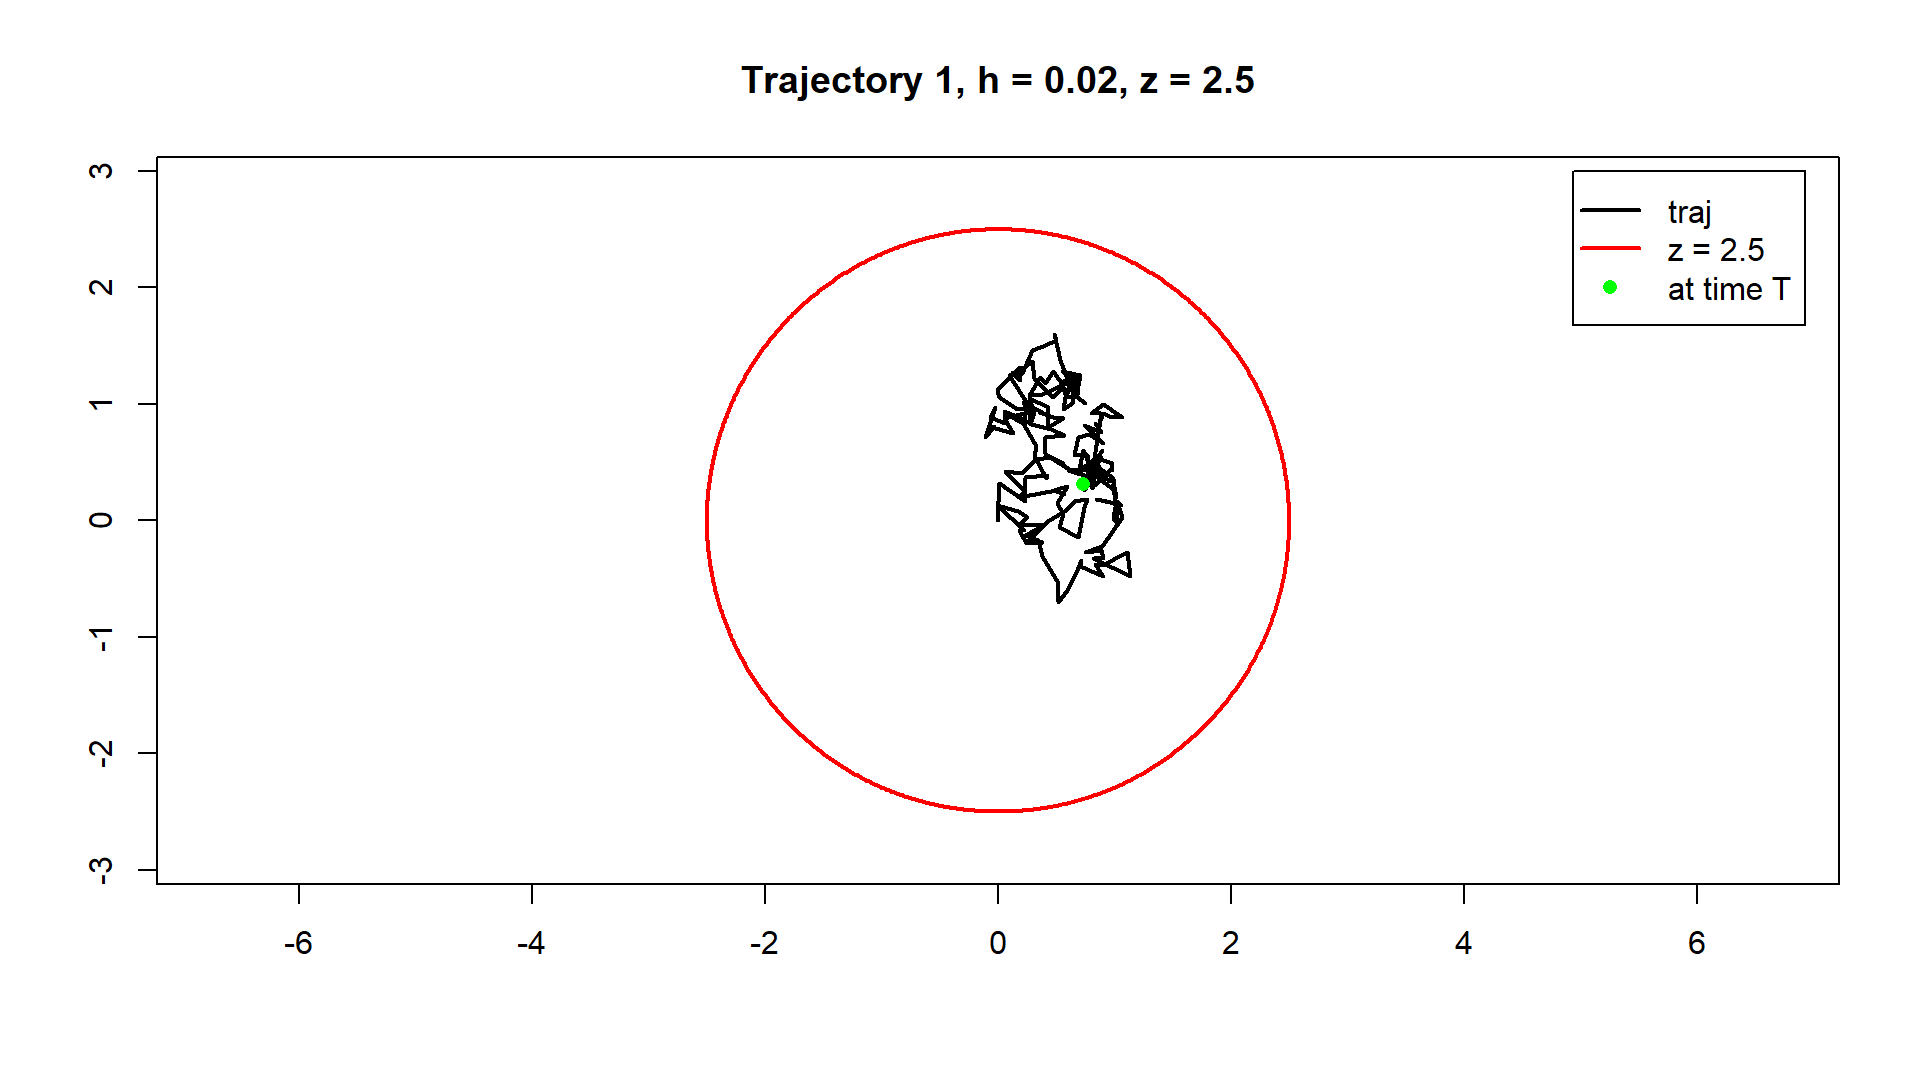
\includegraphics[width=1\linewidth]{../img/2d_1_circle.png}} \\
	\end{minipage}
	\begin{minipage}[h]{1\linewidth}
		\center{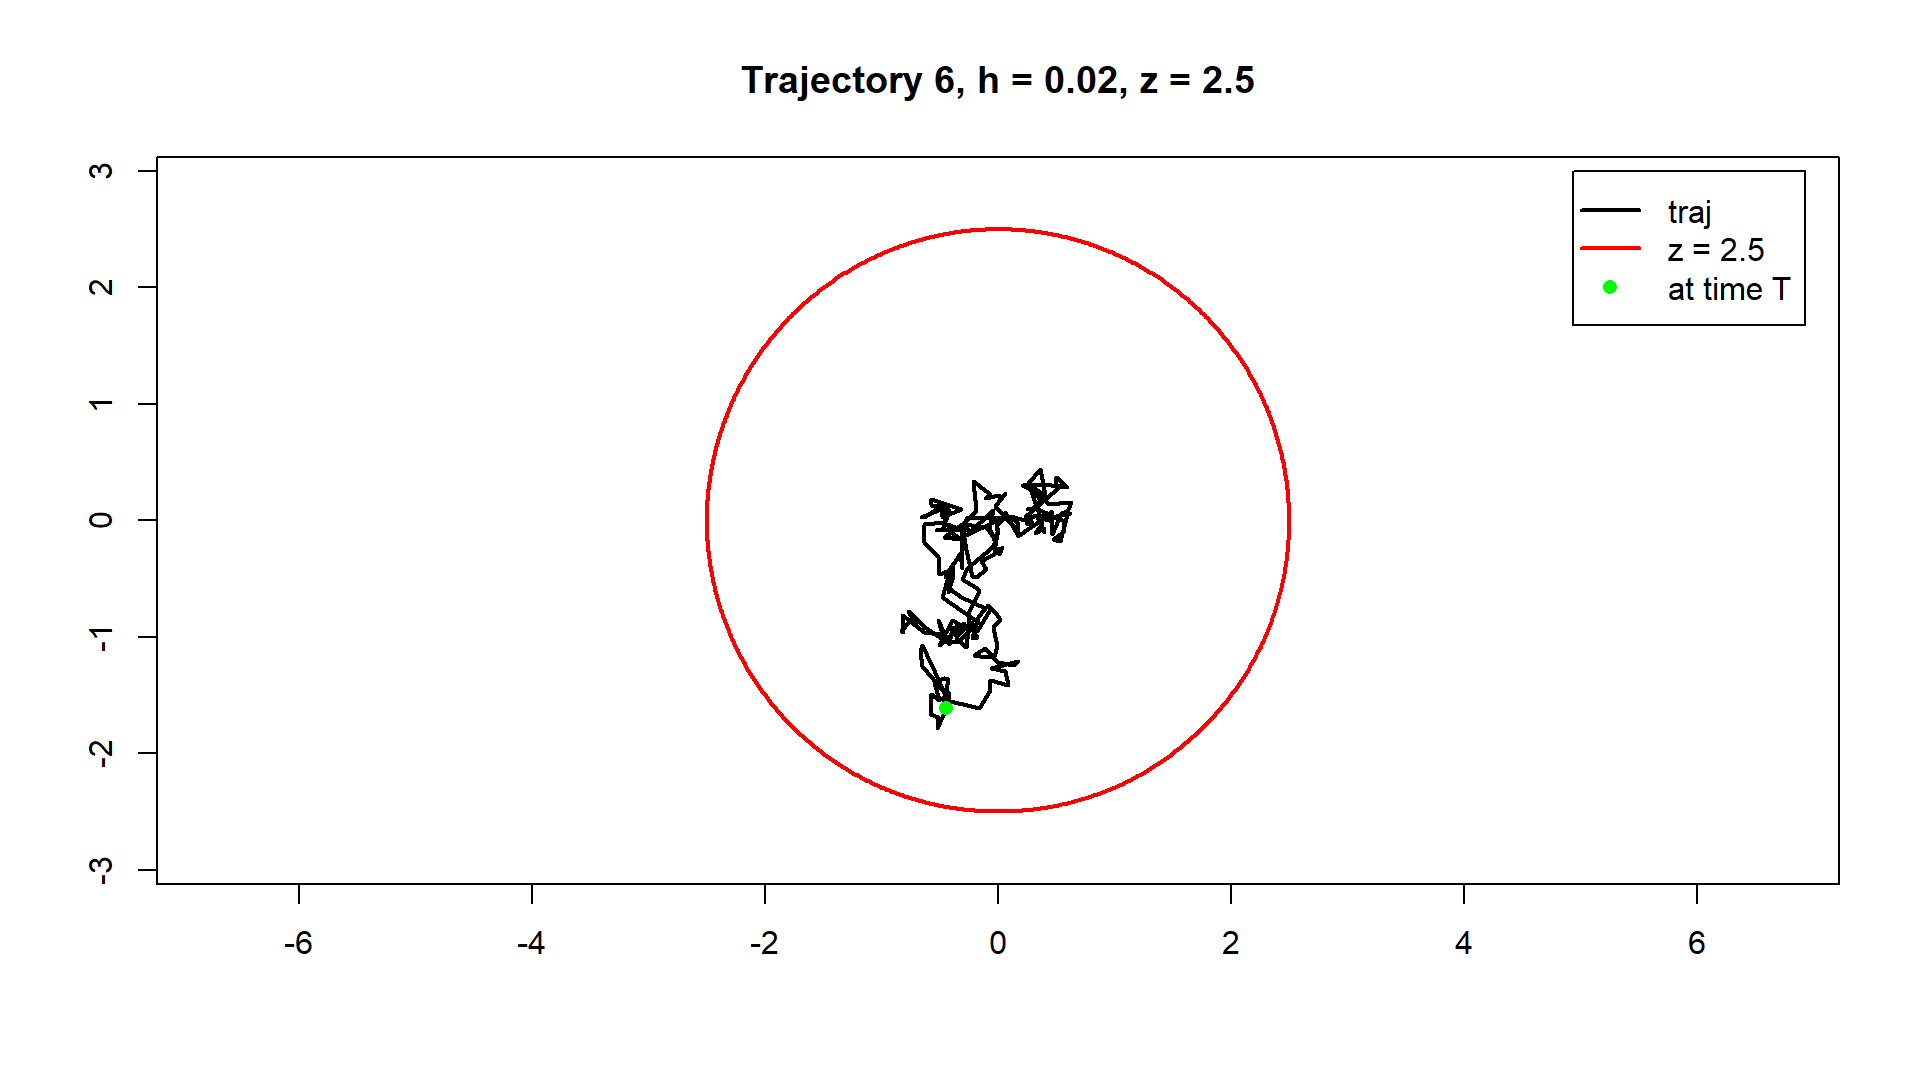
\includegraphics[width=1\linewidth]{../img/2d_6_circle.png}} \\
	\end{minipage}
\end{figure}
\pagebreak
\begin{figure}[H]
	\begin{minipage}[h]{1\linewidth}
		\center{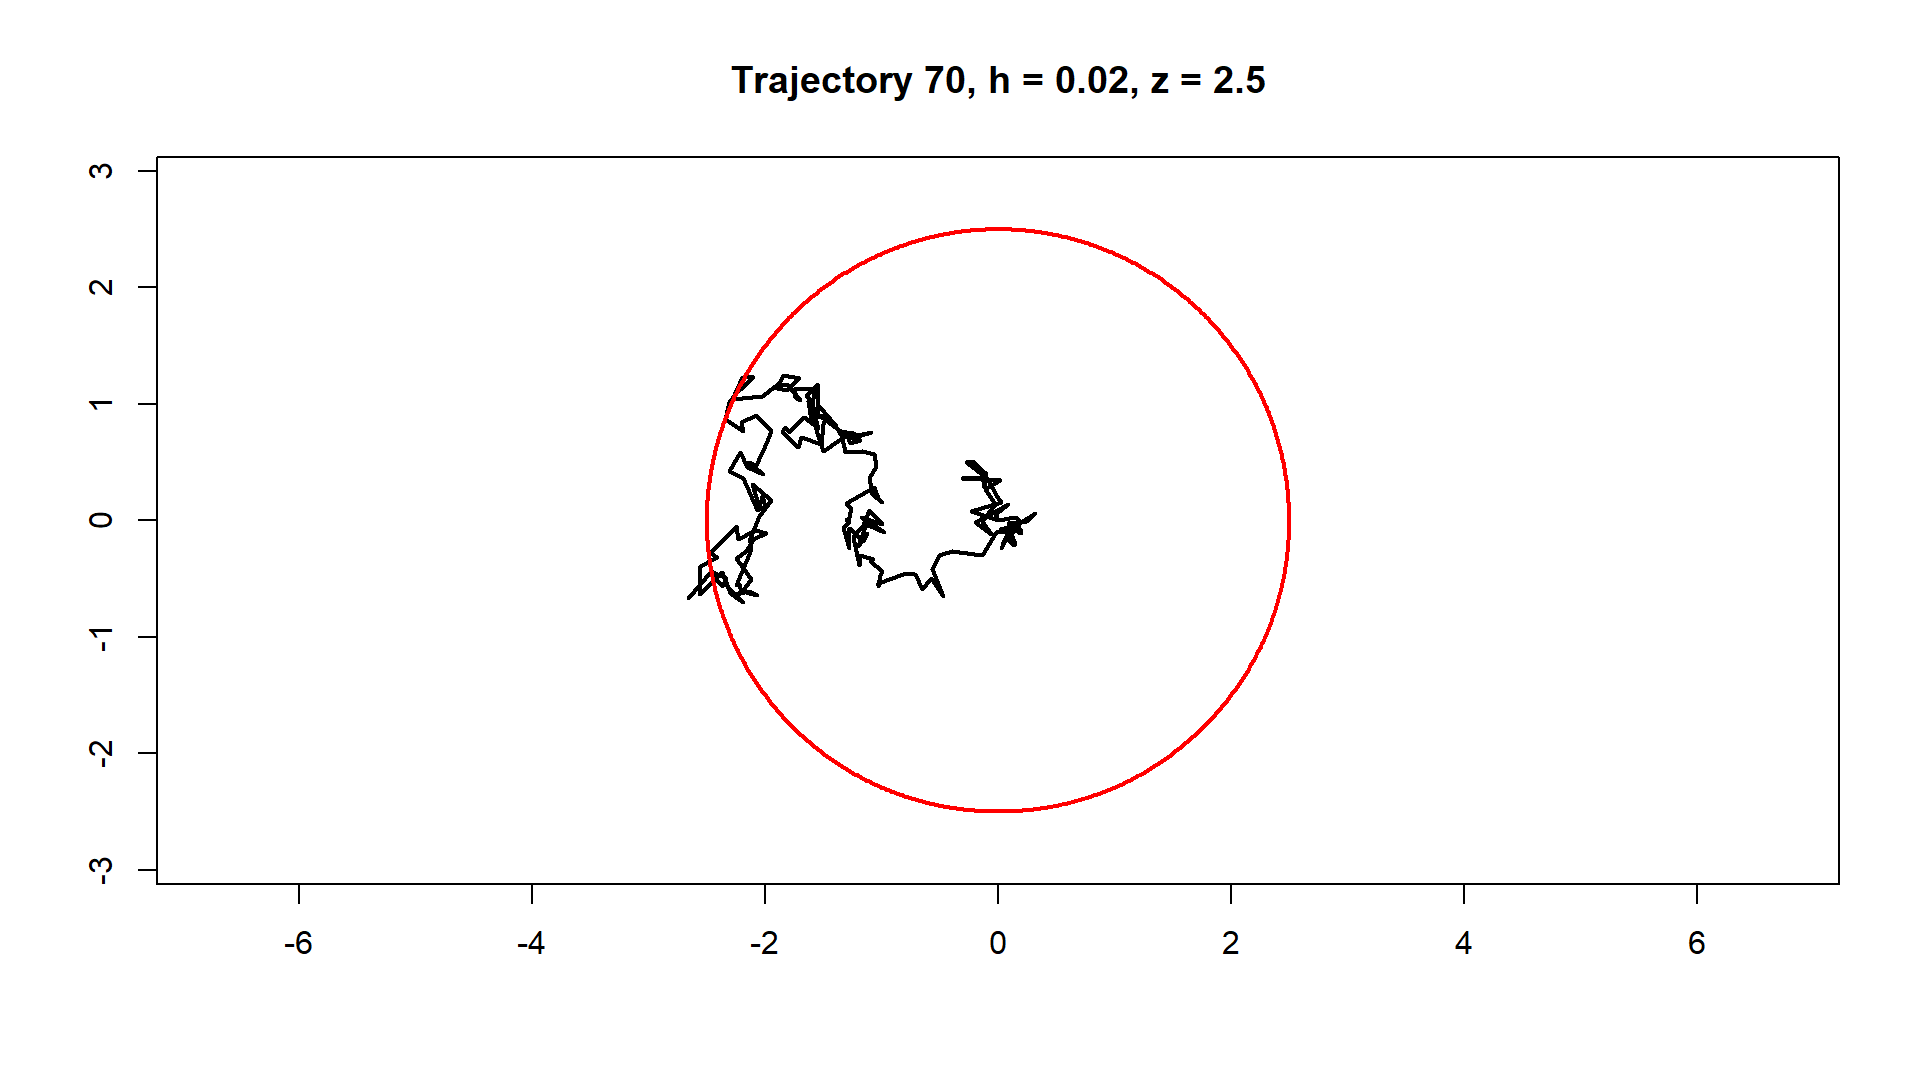
\includegraphics[width=1\linewidth]{../img/2d_70_circle.png}}  \\
	\end{minipage}
	\begin{minipage}[h]{1\linewidth}
		\center{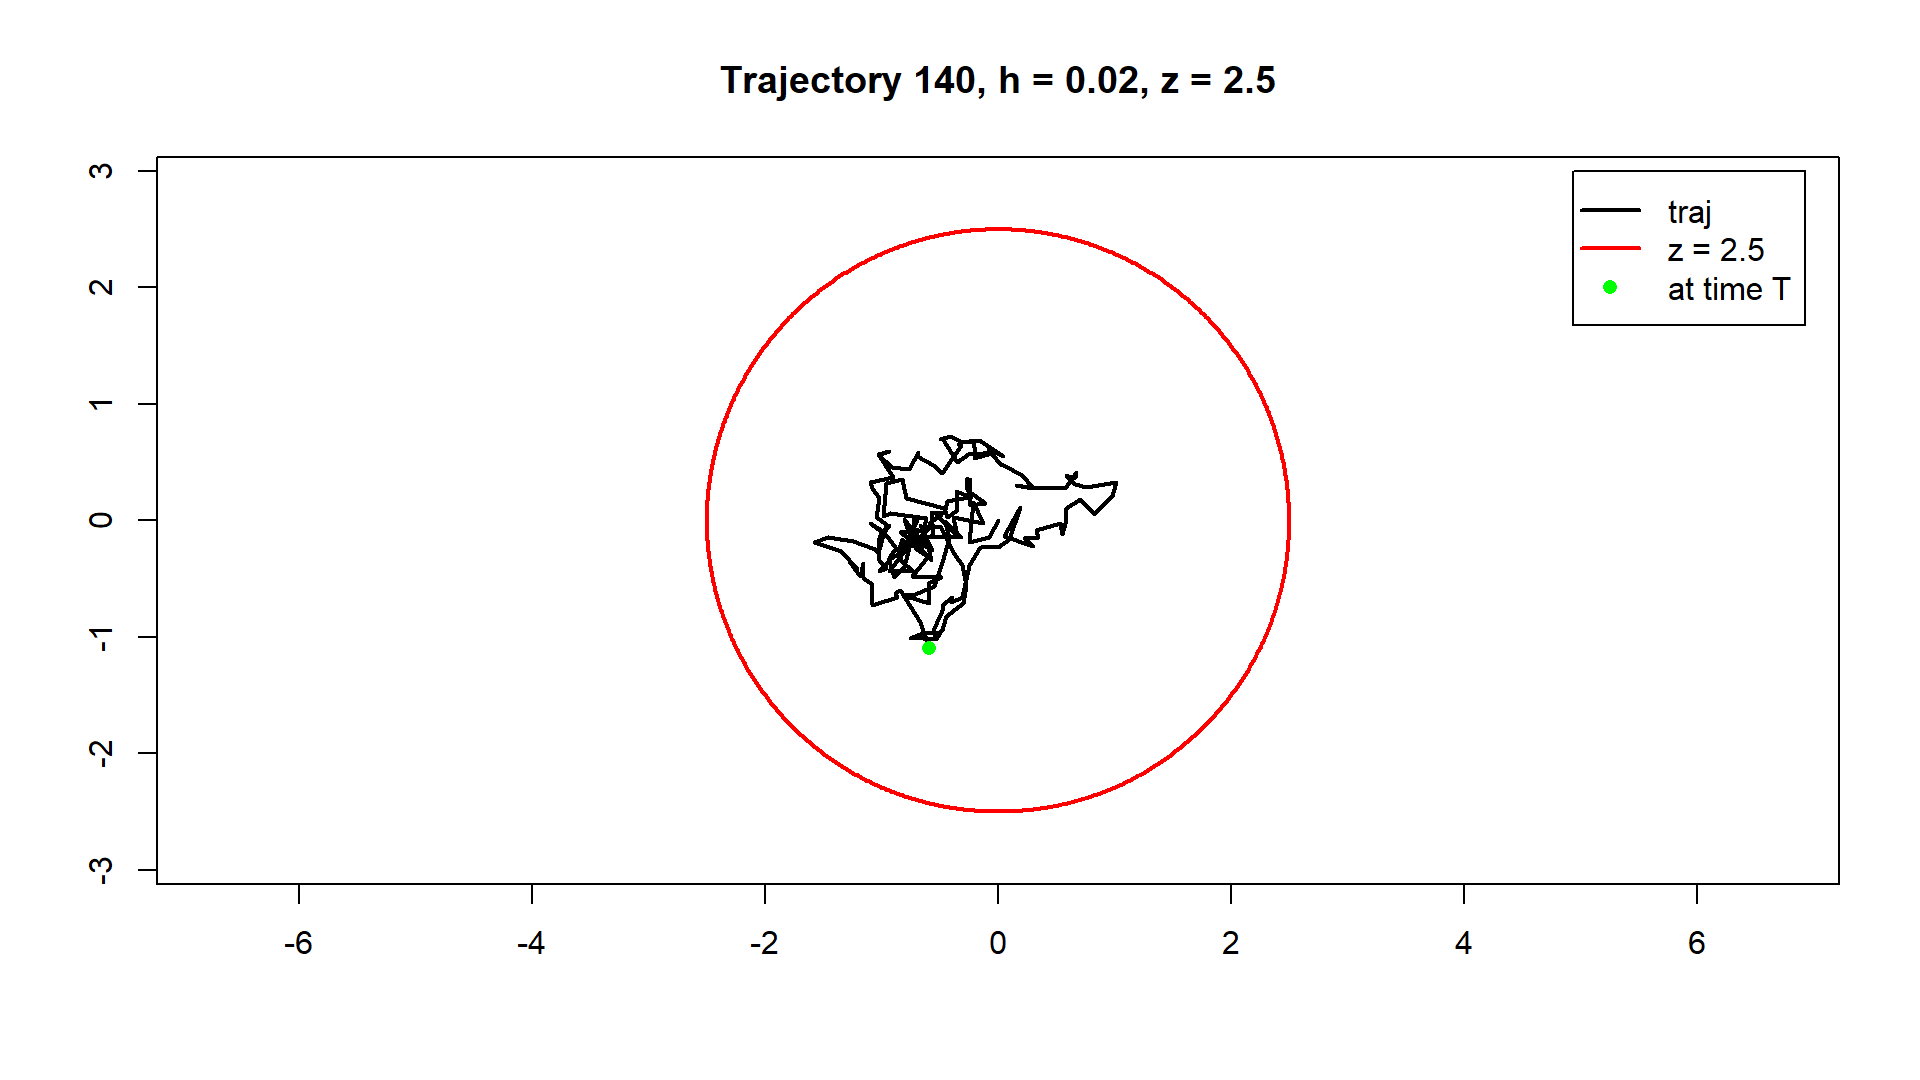
\includegraphics[width=1\linewidth]{../img/2d_140_circle.png}}  \\
	\end{minipage}
\end{figure}










\end{document}